% Options for packages loaded elsewhere
\PassOptionsToPackage{unicode}{hyperref}
\PassOptionsToPackage{hyphens}{url}
\PassOptionsToPackage{dvipsnames,svgnames,x11names}{xcolor}
%
\documentclass[
  a4paper,
]{scrreport}

\usepackage{amsmath,amssymb}
\usepackage{iftex}
\ifPDFTeX
  \usepackage[T1]{fontenc}
  \usepackage[utf8]{inputenc}
  \usepackage{textcomp} % provide euro and other symbols
\else % if luatex or xetex
  \usepackage{unicode-math}
  \defaultfontfeatures{Scale=MatchLowercase}
  \defaultfontfeatures[\rmfamily]{Ligatures=TeX,Scale=1}
\fi
\usepackage{lmodern}
\ifPDFTeX\else  
    % xetex/luatex font selection
\fi
% Use upquote if available, for straight quotes in verbatim environments
\IfFileExists{upquote.sty}{\usepackage{upquote}}{}
\IfFileExists{microtype.sty}{% use microtype if available
  \usepackage[]{microtype}
  \UseMicrotypeSet[protrusion]{basicmath} % disable protrusion for tt fonts
}{}
\makeatletter
\@ifundefined{KOMAClassName}{% if non-KOMA class
  \IfFileExists{parskip.sty}{%
    \usepackage{parskip}
  }{% else
    \setlength{\parindent}{0pt}
    \setlength{\parskip}{6pt plus 2pt minus 1pt}}
}{% if KOMA class
  \KOMAoptions{parskip=half}}
\makeatother
\usepackage{xcolor}
\setlength{\emergencystretch}{3em} % prevent overfull lines
\setcounter{secnumdepth}{5}
% Make \paragraph and \subparagraph free-standing
\makeatletter
\ifx\paragraph\undefined\else
  \let\oldparagraph\paragraph
  \renewcommand{\paragraph}{
    \@ifstar
      \xxxParagraphStar
      \xxxParagraphNoStar
  }
  \newcommand{\xxxParagraphStar}[1]{\oldparagraph*{#1}\mbox{}}
  \newcommand{\xxxParagraphNoStar}[1]{\oldparagraph{#1}\mbox{}}
\fi
\ifx\subparagraph\undefined\else
  \let\oldsubparagraph\subparagraph
  \renewcommand{\subparagraph}{
    \@ifstar
      \xxxSubParagraphStar
      \xxxSubParagraphNoStar
  }
  \newcommand{\xxxSubParagraphStar}[1]{\oldsubparagraph*{#1}\mbox{}}
  \newcommand{\xxxSubParagraphNoStar}[1]{\oldsubparagraph{#1}\mbox{}}
\fi
\makeatother

\usepackage{color}
\usepackage{fancyvrb}
\newcommand{\VerbBar}{|}
\newcommand{\VERB}{\Verb[commandchars=\\\{\}]}
\DefineVerbatimEnvironment{Highlighting}{Verbatim}{commandchars=\\\{\}}
% Add ',fontsize=\small' for more characters per line
\usepackage{framed}
\definecolor{shadecolor}{RGB}{241,243,245}
\newenvironment{Shaded}{\begin{snugshade}}{\end{snugshade}}
\newcommand{\AlertTok}[1]{\textcolor[rgb]{0.68,0.00,0.00}{#1}}
\newcommand{\AnnotationTok}[1]{\textcolor[rgb]{0.37,0.37,0.37}{#1}}
\newcommand{\AttributeTok}[1]{\textcolor[rgb]{0.40,0.45,0.13}{#1}}
\newcommand{\BaseNTok}[1]{\textcolor[rgb]{0.68,0.00,0.00}{#1}}
\newcommand{\BuiltInTok}[1]{\textcolor[rgb]{0.00,0.23,0.31}{#1}}
\newcommand{\CharTok}[1]{\textcolor[rgb]{0.13,0.47,0.30}{#1}}
\newcommand{\CommentTok}[1]{\textcolor[rgb]{0.37,0.37,0.37}{#1}}
\newcommand{\CommentVarTok}[1]{\textcolor[rgb]{0.37,0.37,0.37}{\textit{#1}}}
\newcommand{\ConstantTok}[1]{\textcolor[rgb]{0.56,0.35,0.01}{#1}}
\newcommand{\ControlFlowTok}[1]{\textcolor[rgb]{0.00,0.23,0.31}{\textbf{#1}}}
\newcommand{\DataTypeTok}[1]{\textcolor[rgb]{0.68,0.00,0.00}{#1}}
\newcommand{\DecValTok}[1]{\textcolor[rgb]{0.68,0.00,0.00}{#1}}
\newcommand{\DocumentationTok}[1]{\textcolor[rgb]{0.37,0.37,0.37}{\textit{#1}}}
\newcommand{\ErrorTok}[1]{\textcolor[rgb]{0.68,0.00,0.00}{#1}}
\newcommand{\ExtensionTok}[1]{\textcolor[rgb]{0.00,0.23,0.31}{#1}}
\newcommand{\FloatTok}[1]{\textcolor[rgb]{0.68,0.00,0.00}{#1}}
\newcommand{\FunctionTok}[1]{\textcolor[rgb]{0.28,0.35,0.67}{#1}}
\newcommand{\ImportTok}[1]{\textcolor[rgb]{0.00,0.46,0.62}{#1}}
\newcommand{\InformationTok}[1]{\textcolor[rgb]{0.37,0.37,0.37}{#1}}
\newcommand{\KeywordTok}[1]{\textcolor[rgb]{0.00,0.23,0.31}{\textbf{#1}}}
\newcommand{\NormalTok}[1]{\textcolor[rgb]{0.00,0.23,0.31}{#1}}
\newcommand{\OperatorTok}[1]{\textcolor[rgb]{0.37,0.37,0.37}{#1}}
\newcommand{\OtherTok}[1]{\textcolor[rgb]{0.00,0.23,0.31}{#1}}
\newcommand{\PreprocessorTok}[1]{\textcolor[rgb]{0.68,0.00,0.00}{#1}}
\newcommand{\RegionMarkerTok}[1]{\textcolor[rgb]{0.00,0.23,0.31}{#1}}
\newcommand{\SpecialCharTok}[1]{\textcolor[rgb]{0.37,0.37,0.37}{#1}}
\newcommand{\SpecialStringTok}[1]{\textcolor[rgb]{0.13,0.47,0.30}{#1}}
\newcommand{\StringTok}[1]{\textcolor[rgb]{0.13,0.47,0.30}{#1}}
\newcommand{\VariableTok}[1]{\textcolor[rgb]{0.07,0.07,0.07}{#1}}
\newcommand{\VerbatimStringTok}[1]{\textcolor[rgb]{0.13,0.47,0.30}{#1}}
\newcommand{\WarningTok}[1]{\textcolor[rgb]{0.37,0.37,0.37}{\textit{#1}}}

\providecommand{\tightlist}{%
  \setlength{\itemsep}{0pt}\setlength{\parskip}{0pt}}\usepackage{longtable,booktabs,array}
\usepackage{calc} % for calculating minipage widths
% Correct order of tables after \paragraph or \subparagraph
\usepackage{etoolbox}
\makeatletter
\patchcmd\longtable{\par}{\if@noskipsec\mbox{}\fi\par}{}{}
\makeatother
% Allow footnotes in longtable head/foot
\IfFileExists{footnotehyper.sty}{\usepackage{footnotehyper}}{\usepackage{footnote}}
\makesavenoteenv{longtable}
\usepackage{graphicx}
\makeatletter
\newsavebox\pandoc@box
\newcommand*\pandocbounded[1]{% scales image to fit in text height/width
  \sbox\pandoc@box{#1}%
  \Gscale@div\@tempa{\textheight}{\dimexpr\ht\pandoc@box+\dp\pandoc@box\relax}%
  \Gscale@div\@tempb{\linewidth}{\wd\pandoc@box}%
  \ifdim\@tempb\p@<\@tempa\p@\let\@tempa\@tempb\fi% select the smaller of both
  \ifdim\@tempa\p@<\p@\scalebox{\@tempa}{\usebox\pandoc@box}%
  \else\usebox{\pandoc@box}%
  \fi%
}
% Set default figure placement to htbp
\def\fps@figure{htbp}
\makeatother

%\newfontfamily\Ubuntu[Mapping=tex-text]{Ubuntu}
\usepackage{pgfplots}
\usetikzlibrary{arrows.meta,arrows}
\usetikzlibrary{angles,quotes}
\pgfplotsset{grid style={dashed,mygray}}
% Colors
\definecolor{myblue}{rgb}{0.067,0.529,0.871}
\definecolor{mypurple}{rgb}{0.859,0.071,0.525}
\definecolor{myred}{rgb}{1.0, 0.13, 0.32}
\definecolor{mygreen}{rgb}{0.01, 0.75, 0.24}
\definecolor{myblack}{gray}{0.1}
\definecolor{mygray}{gray}{0.8}
\newcommand{\NN}{\mathbb{N}}
\newcommand{\ZZ}{\mathbb{Z}}
\newcommand{\QQ}{\mathbb{Q}}
\newcommand{\RR}{\mathbb{R}}
\newcommand{\CC}{\mathbb{C}}
\DeclareMathOperator{\operatorname{Int}}{Int}
\DeclareMathOperator{\operatorname{Ext}}{Ext}
\DeclareMathOperator{\operatorname{Fr}}{Fr}
\DeclareMathOperator{\Adh}{Adh}
\DeclareMathOperator{\Ac}{Ac}
\DeclareMathOperator{\sen}{sen}
\usepackage{booktabs}
\usepackage{longtable}
\usepackage{array}
\usepackage{multirow}
\usepackage{wrapfig}
\usepackage{float}
\usepackage{colortbl}
\usepackage{pdflscape}
\usepackage{tabu}
\usepackage{threeparttable}
\usepackage{threeparttablex}
\usepackage[normalem]{ulem}
\usepackage{makecell}
\usepackage{xcolor}
\makeatletter
\@ifpackageloaded{tcolorbox}{}{\usepackage[skins,breakable]{tcolorbox}}
\@ifpackageloaded{fontawesome5}{}{\usepackage{fontawesome5}}
\definecolor{quarto-callout-color}{HTML}{909090}
\definecolor{quarto-callout-note-color}{HTML}{0758E5}
\definecolor{quarto-callout-important-color}{HTML}{CC1914}
\definecolor{quarto-callout-warning-color}{HTML}{EB9113}
\definecolor{quarto-callout-tip-color}{HTML}{00A047}
\definecolor{quarto-callout-caution-color}{HTML}{FC5300}
\definecolor{quarto-callout-color-frame}{HTML}{acacac}
\definecolor{quarto-callout-note-color-frame}{HTML}{4582ec}
\definecolor{quarto-callout-important-color-frame}{HTML}{d9534f}
\definecolor{quarto-callout-warning-color-frame}{HTML}{f0ad4e}
\definecolor{quarto-callout-tip-color-frame}{HTML}{02b875}
\definecolor{quarto-callout-caution-color-frame}{HTML}{fd7e14}
\makeatother
\makeatletter
\@ifpackageloaded{bookmark}{}{\usepackage{bookmark}}
\makeatother
\makeatletter
\@ifpackageloaded{caption}{}{\usepackage{caption}}
\AtBeginDocument{%
\ifdefined\contentsname
  \renewcommand*\contentsname{Tabla de contenidos}
\else
  \newcommand\contentsname{Tabla de contenidos}
\fi
\ifdefined\listfigurename
  \renewcommand*\listfigurename{Listado de Figuras}
\else
  \newcommand\listfigurename{Listado de Figuras}
\fi
\ifdefined\listtablename
  \renewcommand*\listtablename{Listado de Tablas}
\else
  \newcommand\listtablename{Listado de Tablas}
\fi
\ifdefined\figurename
  \renewcommand*\figurename{Figura}
\else
  \newcommand\figurename{Figura}
\fi
\ifdefined\tablename
  \renewcommand*\tablename{Tabla}
\else
  \newcommand\tablename{Tabla}
\fi
}
\@ifpackageloaded{float}{}{\usepackage{float}}
\floatstyle{ruled}
\@ifundefined{c@chapter}{\newfloat{codelisting}{h}{lop}}{\newfloat{codelisting}{h}{lop}[chapter]}
\floatname{codelisting}{Listado}
\newcommand*\listoflistings{\listof{codelisting}{Listado de Listados}}
\usepackage{amsthm}
\theoremstyle{definition}
\newtheorem{exercise}{Ejercicio}[chapter]
\theoremstyle{remark}
\AtBeginDocument{\renewcommand*{\proofname}{Prueba}}
\newtheorem*{remark}{Observación}
\newtheorem*{solution}{Solución}
\newtheorem{refremark}{Observación}[chapter]
\newtheorem{refsolution}{Solución}[chapter]
\makeatother
\makeatletter
\makeatother
\makeatletter
\@ifpackageloaded{caption}{}{\usepackage{caption}}
\@ifpackageloaded{subcaption}{}{\usepackage{subcaption}}
\makeatother

\ifLuaTeX
\usepackage[bidi=basic]{babel}
\else
\usepackage[bidi=default]{babel}
\fi
\babelprovide[main,import]{spanish}
% get rid of language-specific shorthands (see #6817):
\let\LanguageShortHands\languageshorthands
\def\languageshorthands#1{}
\usepackage{bookmark}

\IfFileExists{xurl.sty}{\usepackage{xurl}}{} % add URL line breaks if available
\urlstyle{same} % disable monospaced font for URLs
\hypersetup{
  pdftitle={Problemas de Bioestadística},
  pdfauthor={Alfredo Sánchez Alberca},
  pdflang={es},
  colorlinks=true,
  linkcolor={blue},
  filecolor={Maroon},
  citecolor={Blue},
  urlcolor={Blue},
  pdfcreator={LaTeX via pandoc}}


\title{Problemas de Bioestadística}
\author{Alfredo Sánchez Alberca}
\date{2022-01-06}

\begin{document}
\begin{titlepage}

%\AddToShipoutPicture*{\put(0,0){\includegraphics[scale=0.8]{img/background2}}} % Imagen de fondo, requiere el paquete eso-pic.
\begin{center}
\vspace*{5cm}

\Huge
{\textbf{\textsf{Problemas de Bioestadística}}}

\vspace{0.5cm}
\LARGE
{\textbf{\textsf{}}}

\vspace{1.5cm}


\includegraphics[width=0.4\textwidth]{img/logos/sticker.png}
\end{center}

\vfill

\begin{flushleft}
\begin{tabular}{ll}

\includegraphics[width=0.1\textwidth]{img/logos/aprendeconalf.png} & \parbox[b]{5cm}{\Large\textsf{Alfredo
Sánchez
Alberca}\\ \textsf{asalber@ceu.es} \\ \textsf{https://aprendeconalf.es}}
\end{tabular}
\end{flushleft}
\end{titlepage}
\renewcommand*\contentsname{Tabla de contenidos}
{
\hypersetup{linkcolor=}
\setcounter{tocdepth}{2}
\tableofcontents
}

\bookmarksetup{startatroot}

\chapter*{Prefacio}\label{prefacio}
\addcontentsline{toc}{chapter}{Prefacio}

\markboth{Prefacio}{Prefacio}

Colección de problemas de Bioestadística para el Master en
Nutrigenómica.

\bookmarksetup{startatroot}

\chapter{Contrastes de hipótesis
paramétricos}\label{contrastes-de-hipuxf3tesis-paramuxe9tricos}

\begin{exercise}[]\protect\hypertarget{exr-contraste-media-consumo-azucar}{}\label{exr-contraste-media-consumo-azucar}

Sabiendo que el año pasado el consumo per cápita de azúcar en España fue
de \(4.8\) kg y que este consumo sigue una distribución normal, hemos
seleccionado aleatoriamente a \(20\) españoles obteniendo una media
muestral de \(5\) kg y una cuasidesviación típica muestral de \(0.4\)
kg. Contrastar la hipótesis de que el consumo de azúcar per cápita de
este año en España no ha variado utilizando un nivel de significación
del \(10\)\%.

\end{exercise}

\begin{tcolorbox}[enhanced jigsaw, breakable, opacityback=0, colbacktitle=quarto-callout-tip-color!10!white, colframe=quarto-callout-tip-color-frame, left=2mm, titlerule=0mm, coltitle=black, colback=white, bottomtitle=1mm, toptitle=1mm, opacitybacktitle=0.6, title=\textcolor{quarto-callout-tip-color}{\faLightbulb}\hspace{0.5em}{Solución}, leftrule=.75mm, bottomrule=.15mm, toprule=.15mm, rightrule=.15mm, arc=.35mm]

Sea \(X\sim N(\mu,\sigma)\) la variable aleatoria que mide el consumo
per cápita de azúcar en España.\\
Número de poblaciones: 1 población. Variable dependiente: Consumo de
azúcar (cuantitativa).\\
Tamaño muestral: \(n=20\).\\
Contraste de la media de una población normal (prueba t):
\(H_0:\mu=4.8\), \(H_1:\mu\neq 4.8\).\\
Estadístico del contraste: \(t=2.24\)\\
p-valor: \(p =2 P(t(19)>2.24) = 0.037\).\\
Como el p-valor es menor que el nivel de significación \(\alpha = 0.1\),
se rechaza la hipótesis nula y se concluye que el consumo de azúcar per
cápita de este año en España ha variado.

\end{tcolorbox}

\begin{exercise}[]\protect\hypertarget{exr-contraste-proporcion-bolleria-industrial}{}\label{exr-contraste-proporcion-bolleria-industrial}

En una clase de alumnos de primaria se ha comprobado que el \(20\)\% del
alumnado consume bollería industrial. Para disminuir esta preocupante
cifra, el colegio ha implantado un programa de educación nutricional.
Después del programa se tomó una muestra aleatoria de \(50\) alumnos de
primaria y se observó que 8 seguían consumiendo bollería industrial.
Contrastar con un nivel de significación del \(5\)\% si el programa es
efectivo.

\end{exercise}

\begin{tcolorbox}[enhanced jigsaw, breakable, opacityback=0, colbacktitle=quarto-callout-tip-color!10!white, colframe=quarto-callout-tip-color-frame, left=2mm, titlerule=0mm, coltitle=black, colback=white, bottomtitle=1mm, toptitle=1mm, opacitybacktitle=0.6, title=\textcolor{quarto-callout-tip-color}{\faLightbulb}\hspace{0.5em}{Solución}, leftrule=.75mm, bottomrule=.15mm, toprule=.15mm, rightrule=.15mm, arc=.35mm]

Número de poblaciones: 1 población.\\
Variable dependiente: Consumo de bollería industrial (cualitativa
binaria).\\
Tamaño muestral: \(n=50\).\\
Contraste para la proporción de una población: \(H_0:p=0.2\),
\(H_1:p< 0.2\).\\
p-valor: \(p=0.2979\).\\
Como el p-valor es mayor que el nivel de significación
\(\alpha = 0.05\), no se rechaza la hipótesis nula y se concluye que no
hay evidencias significativas de que el programa sea efectivo.

\end{tcolorbox}

\begin{exercise}[]\protect\hypertarget{exr-contraste-media-consumo}{}\label{exr-contraste-media-consumo}

Se sabe que el consumo anual de helado correspondiente a cada español
sigue una distribución normal y que el año pasado el consumo medio fue
de 20 kg. Queremos contrastar si este año se va a mantener el consumo
medio de helado que el año pasado, y para comprobarlo se efectúa una
muestra aleatoria de 22 españoles, obteniéndose los resultados recogidos
en el fichero \href{datos/consumo-helado.csv}{consumo-helado.csv}.
Realizar el contraste con un nivel de significación de \(0.10\).

\end{exercise}

\begin{tcolorbox}[enhanced jigsaw, breakable, opacityback=0, colbacktitle=quarto-callout-tip-color!10!white, colframe=quarto-callout-tip-color-frame, left=2mm, titlerule=0mm, coltitle=black, colback=white, bottomtitle=1mm, toptitle=1mm, opacitybacktitle=0.6, title=\textcolor{quarto-callout-tip-color}{\faLightbulb}\hspace{0.5em}{Solución}, leftrule=.75mm, bottomrule=.15mm, toprule=.15mm, rightrule=.15mm, arc=.35mm]

Número de poblaciones: 1 población.\\
Variable dependiente: Consumo de helado (cuantitativa).\\
Tamaño muestral: \(n=22\).\\
Prueba de normalidad de Kolmogorov-Smirnov. p-valor: \(p=0.632\). Se
acepta la normalidad.\\
Contraste de la media de una población normal (prueba t):
\(H_0:\mu=20\), \(H_1:\mu\neq 20\).\\
p-valor: \(p = 0.8033\).\\
Como el p-valor es mayor que el nivel de significación
\(\alpha = 0.10\), no se rechaza la hipótesis nula y se concluye que el
consumo medio de helado de este año en España se va a mantener.

\end{tcolorbox}

\begin{exercise}[]\protect\hypertarget{exr-contraste-comparacion-medias-pareadas-hierro}{}\label{exr-contraste-comparacion-medias-pareadas-hierro}

Se ha realizado un estudio para comparar los niveles de hierro en sangre
antes y después de un programa de ejercicios. Los datos del estudio
están en el fichero
\href{datos/niveles-hierro-ejercicio.csv}{niveles-hierro-ejercicio.csv}.
Realizar el contraste de hipótesis adecuado para ver si el ejercicio
aumenta el nivel de hierro con un nivel de significación del 1\%.

\end{exercise}

\begin{tcolorbox}[enhanced jigsaw, breakable, opacityback=0, colbacktitle=quarto-callout-tip-color!10!white, colframe=quarto-callout-tip-color-frame, left=2mm, titlerule=0mm, coltitle=black, colback=white, bottomtitle=1mm, toptitle=1mm, opacitybacktitle=0.6, title=\textcolor{quarto-callout-tip-color}{\faLightbulb}\hspace{0.5em}{Solución}, leftrule=.75mm, bottomrule=.15mm, toprule=.15mm, rightrule=.15mm, arc=.35mm]

Número de poblaciones: 2 poblaciones pareadas (población 1: antes de
hacer ejercicio, población 2: después de hacer ejercicio).\\
Variable dependiente: Nivel de hierro (cuantitativa).\\
Tamaño muestral: \(n=20\).\\
Prueba de normalidad de Kolmogorov-Smirnov: p-valor de la diferencia:
\(0.804\). Se acepta la normalidad.\\
Contraste para la comparación de medias de poblaciones pareadas:
\(H_0:\mu_d=0\), \(H_1:\mu_d< 0\).\\
p-valor: \(p=0.0011\).\\
Como el p-valor es menor que el nivel de significación se rechaza la
hipótesis nula y se concluye que el programa de ejercicios ha aumentado
significativamente el nivel de hierro en sangre.

\end{tcolorbox}

\begin{exercise}[]\protect\hypertarget{exr-contraste-comparacion-medias-glucosa}{}\label{exr-contraste-comparacion-medias-glucosa}

Se ha realizado un estudio para comparar los niveles de glucosa en
sangre de dos grupos: uno sigue una dieta baja en carbohidratos y otro
una dieta estándar. Los datos del estudio están en el fichero
\href{datos/niveles-glucosa-dietas.csv}{niveles-glucosa-dietas.csv}.
Realizar el contraste de hipótesis adecuado para comparar las medias de
los dos grupos con un nivel de significación del 5\%.

\end{exercise}

\begin{tcolorbox}[enhanced jigsaw, breakable, opacityback=0, colbacktitle=quarto-callout-tip-color!10!white, colframe=quarto-callout-tip-color-frame, left=2mm, titlerule=0mm, coltitle=black, colback=white, bottomtitle=1mm, toptitle=1mm, opacitybacktitle=0.6, title=\textcolor{quarto-callout-tip-color}{\faLightbulb}\hspace{0.5em}{Solución}, leftrule=.75mm, bottomrule=.15mm, toprule=.15mm, rightrule=.15mm, arc=.35mm]

Número de poblaciones: 2 poblaciones independientes (población 1: dieta
baja en carbohidratos, población 2: dieta estándar).\\
Variable dependiente: Nivel de glucosa (cuantitativa).\\
Tamaños muestrales: \(n_1=30\), \(n_2=30\).\\
Contraste de comparación de varianzas: \(H_0:\sigma_1^2=\sigma_2^2\),
\(H_1:\sigma_1^2\neq \sigma_2^2\). p-valor: \(p=0.25\). Se acepta la
hipótesis nula de igualdad de varianzas.\\
Contraste para la comparación de medias de poblaciones independientes
con varianzas iguales: \(H_0:\mu_1=\mu_2\), \(H_1:\mu_1<\mu_2\).\\
p-valor: \(p=0.00009\). Como el p-valor es menor que el nivel de
significación se rechaza la hipótesis nula y se concluye que el nivel de
glucosa en sangre es significativamente menor en el grupo que sigue una
dieta baja en carbohidratos.

\end{tcolorbox}

\begin{exercise}[]\protect\hypertarget{exr-contraste-comparacion-medias-expresion-genica}{}\label{exr-contraste-comparacion-medias-expresion-genica}

Se ha realizado un estudio para comparar los niveles de expresión de un
gen en función de la dieta (vegetariana u omnívora). Los datos del
estudio están en el fichero
\href{datos/expresion-genica-dietas.csv}{expresion-genica-dietas.csv}.
Realizar el contraste de hipótesis adecuado para comparar las medias de
los dos grupos.

\end{exercise}

\begin{tcolorbox}[enhanced jigsaw, breakable, opacityback=0, colbacktitle=quarto-callout-tip-color!10!white, colframe=quarto-callout-tip-color-frame, left=2mm, titlerule=0mm, coltitle=black, colback=white, bottomtitle=1mm, toptitle=1mm, opacitybacktitle=0.6, title=\textcolor{quarto-callout-tip-color}{\faLightbulb}\hspace{0.5em}{Solución}, leftrule=.75mm, bottomrule=.15mm, toprule=.15mm, rightrule=.15mm, arc=.35mm]

Número de poblaciones: 2 poblaciones independientes (población 1: dieta
vegetariana, población 2: dieta omnívora).\\
Variable dependiente: Expresión génica (cuantitativa).\\
Tamaños muestrales: \(n_1=20\), \(n_2=25\).\\
Prueba de normalidad de Kolmogorov-Smirnov: p-valor primera muestra:
\(0.4164\), p-valor segunda muestra: \(0.2767\). Se acepta la normalidad
en ambos grupos.\\
Contraste de comparación de varianzas: \(H_0:\sigma_1^2=\sigma_2^2\),
\(H_1:\sigma_1^2\neq \sigma_2^2\). p-valor: \(p=0.1373\). Se acepta la
hipótesis nula de igualdad de varianzas.\\
Contraste para la comparación de medias de poblaciones independientes
con varianzas iguales: \(H_0:\mu_1=\mu_2\), \(H_1:\mu_1<\mu_2\).\\
p-valor: \(p=0.00006\).\\
Como el p-valor es menor que el nivel de significación, se rechaza la
hipótesis nula y se concluye que existen diferencias estadísticamente
significativas en los niveles de expresión génica en función de la
dieta.

\end{tcolorbox}

\begin{exercise}[]\protect\hypertarget{exr-contraste-comparacion-proporciones-vitamina-c}{}\label{exr-contraste-comparacion-proporciones-vitamina-c}

Se utiliza un grupo de 150 pacientes para comprobar la teoría de que la
vitamina C tiene alguna influencia en el tratamiento del cáncer. Los 150
pacientes fueron divididos en dos grupos de 75. Un grupo recibió 10
gramos de vitamina C y el otro un placebo cada día, además de la
medicación habitual. De los que recibieron la vitamina C, 47 presentaban
alguna mejoría al cabo de cuatro semanas, mientras que de los que
recibieron el placebo, 43 experimentaron mejoría. Contrastar la
hipótesis de que la vitamina C tiene influencia en el tratamiento del
cáncer con un nivel de significación del 5\%.

\end{exercise}

\begin{tcolorbox}[enhanced jigsaw, breakable, opacityback=0, colbacktitle=quarto-callout-tip-color!10!white, colframe=quarto-callout-tip-color-frame, left=2mm, titlerule=0mm, coltitle=black, colback=white, bottomtitle=1mm, toptitle=1mm, opacitybacktitle=0.6, title=\textcolor{quarto-callout-tip-color}{\faLightbulb}\hspace{0.5em}{Solución}, leftrule=.75mm, bottomrule=.15mm, toprule=.15mm, rightrule=.15mm, arc=.35mm]

Número de poblaciones: 2 poblaciones independientes (población 1:
vitamina C, población 2: placebo).\\
Variable dependiente: Mejoría en el tratamiento del cáncer (cualitativa
binaria).\\
Tamaños muestrales: \(n_1=75\), \(n_2=75\).\\
Contraste para la comparación de proporciones: \(H_0:p_1=p_2\),
\(H_1:p_1\neq p_2\).\\
p-valor: \(p=0.6824\).\\
Como el p-valor es mayor que el nivel de significación, no se rechaza la
hipótesis nula y se concluye que no hay evidencias significativas de que
la vitamina C tenga influencia en el tratamiento del cáncer.

\end{tcolorbox}

\begin{exercise}[]\protect\hypertarget{exr-contraste-proporcion-consumo-alcohol}{}\label{exr-contraste-proporcion-consumo-alcohol}

En un estudio sobre el consumo de alcohol entre los jóvenes durante los
fines de semana, se preguntó a 100 chicos y a 125 chicas, de los que 63
chicos y 59 chicas contestaron que consumían. En vista de estos datos,
¿existe alguna diferencia significativa entre las proporciones de chicos
y chicas que consumen alcohol los fines de semana?

\end{exercise}

\begin{tcolorbox}[enhanced jigsaw, breakable, opacityback=0, colbacktitle=quarto-callout-tip-color!10!white, colframe=quarto-callout-tip-color-frame, left=2mm, titlerule=0mm, coltitle=black, colback=white, bottomtitle=1mm, toptitle=1mm, opacitybacktitle=0.6, title=\textcolor{quarto-callout-tip-color}{\faLightbulb}\hspace{0.5em}{Solución}, leftrule=.75mm, bottomrule=.15mm, toprule=.15mm, rightrule=.15mm, arc=.35mm]

Número de poblaciones: 2 poblaciones independientes (población 1:
chicos, población 2: chicas).\\
Variable dependiente: Consumo de alcohol (cualitativa binaria).\\
Tamaños muestrales: \(n_1=100\), \(n_2=125\).\\
Contraste para la comparación de proporciones: \(H_0:p_1=p_2\),
\(H_1:p_1\neq p_2\).\\
p-valor: \(p=0.0163\).\\
Como el p-valor es menor que el nivel de significación, se rechaza la
hipótesis nula y se concluye que hay diferencias significativas entre el
consumo de alcohol de chicos y chicas.

\end{tcolorbox}

\begin{exercise}[]\protect\hypertarget{exr-contraste-anova-suplementacion}{}\label{exr-contraste-anova-suplementacion}

En un estudio de genómica nutricional, se evalúa cómo afecta la
suplementación con diferentes tipos de macronutrientes a la expresión de
un gen relacionado con el metabolismo energético. Los investigadores
dividen a los participantes en tres grupos, cada uno recibiendo una
dieta suplementada (1 carbohidratos, 2 proteínas y 3 grasas).Se mide el
nivel de expresión génica (ΔCt, relativo a un gen de referencia) en 25
individuos por grupo. Los resultados se recogen en el fichero
\href{datos/expresion-genica-suplementacion.csv}{expresion-genica-suplementacion.csv}.
Realizar el contraste de hipótesis adecuado para comparar ver si hay
diferencias estadísticamente significativas entre las expresiones
génicas de los tres grupos.

\end{exercise}

\begin{tcolorbox}[enhanced jigsaw, breakable, opacityback=0, colbacktitle=quarto-callout-tip-color!10!white, colframe=quarto-callout-tip-color-frame, left=2mm, titlerule=0mm, coltitle=black, colback=white, bottomtitle=1mm, toptitle=1mm, opacitybacktitle=0.6, title=\textcolor{quarto-callout-tip-color}{\faLightbulb}\hspace{0.5em}{Solución}, leftrule=.75mm, bottomrule=.15mm, toprule=.15mm, rightrule=.15mm, arc=.35mm]

Número de poblaciones: 3 poblaciones independientes (población 1:
Carbohidratos, población 2: Proteínas, población 3: Grasas).\\
Variable dependiente: Expresión génica (cuantitativa).\\
Tamaños muestrales: \(n_1=75\), \(n_2=75\) y \(n_3=75\).\\
Contraste de normalidad de Kolmogorov-Smirnov: p-valor primera muestra:
\(0.7571\), p-valor segunda muestra: \(0.6459\), p-valor tercera
muestra: \(0.9643\). Se acepta la normalidad en los tres grupos.\\
Contraste de homocedasticidad de Levene: p-valor: \(0.2126\). Se acepta
la hipótesis de igualdad de varianzas.\\
Contraste de ANOVA: \(H_0:\mu_1=\mu_2=\mu_3\), \(H_1:\) Al menos dos
medias son diferentes.\\
p-valor: \(p=0.000283\).\\
Como el p-valor es menor que el nivel de significación, se rechaza la
hipótesis nula y se concluye que hay diferencias significativas entre
las medias de la expresión génica de los grupos de suplementación.\\
Contraste post hoc de Tukey:\\
- Carbohidratos vs Proteínas: \(p=0.0016\). Hay diferencias
significativas.\\
- Carbohidratos vs Grasas: \(p=0.0009\). Hay diferencias
significativas.\\
- Proteínas vs Grasas: \(p=0.9809\). No hay diferencias significativas.

\end{tcolorbox}

\begin{exercise}[]\protect\hypertarget{exr-contraste-anova-interaccion-dieta-farmaco}{}\label{exr-contraste-anova-interaccion-dieta-farmaco}

En un estudio diseñado para analizar la influencia de un tipo de dieta y
de un fármaco en el peso corporal perdido, se ha anotado el número de Kg
perdidos en un grupo de personas al cabo de 3 meses de dieta y de tomar
el fármaco en el fichero
\href{datos/interaccion-dieta-farmaco.csv}{interaccion-dieta-farmaco.csv}.
Realizar el contraste de hipótesis adecuado para ver si el peso perdido
depende de la dieta, del fármaco y de la interacción entre ambos.

\end{exercise}

\begin{tcolorbox}[enhanced jigsaw, breakable, opacityback=0, colbacktitle=quarto-callout-tip-color!10!white, colframe=quarto-callout-tip-color-frame, left=2mm, titlerule=0mm, coltitle=black, colback=white, bottomtitle=1mm, toptitle=1mm, opacitybacktitle=0.6, title=\textcolor{quarto-callout-tip-color}{\faLightbulb}\hspace{0.5em}{Solución}, leftrule=.75mm, bottomrule=.15mm, toprule=.15mm, rightrule=.15mm, arc=.35mm]

Número de poblaciones: 4 poblaciones independientes (población 1: Dieta
No + Fármaco No, población 2: Dieta No + Fármaco Si, población 3: Dieta
Si + Fármaco No, población 4: Dieta Si + Fármaco Si).\\
Variable dependiente: Peso perdido (cuantitativa).\\
Tamaños muestrales: \(n_1=5\), \(n_2=6\), \(n_3=5\) y \(n_4=6\).\\
Contraste de normalidad de Shapiro-Wilk: p-valor primera muestra:
\(0.4677\), p-valor segunda muestra: \(0.9672\), p-valor tercera
muestra: \(0.741\), p-valor cuarta muestra: \(0.719\). Se acepta la
normalidad en los cuatro grupos.\\
Contraste de homocedasticidad de Levene: p-valor: \(0.845\). Se acepta
la hipótesis de igualdad de varianzas.\\
Contraste de ANOVA de dos factores con interacción: \(H_0:\) No hay
interacción entre la dieta y el fármaco, \(H_1:\) Hay interacción entre
la dieta y el fármaco.\\
- p-valor dieta: \(p=0.0000\).\\
- p-valor fármaco: \(p=0.0000\).\\
- p-valor interacción: \(p=0.0012\).\\
Como el p-valor es menor que el nivel de significación en los tres
casos, se rechaza la hipótesis nula y se concluye que la pérdida de peso
depende de la dieta, del fármaco y de la interacción entre ambos.

\end{tcolorbox}

\bookmarksetup{startatroot}

\chapter{Prácticas de contrastes de hipótesis paramétricos con
R}\label{pruxe1cticas-de-contrastes-de-hipuxf3tesis-paramuxe9tricos-con-r}

\begin{exercise}[]\protect\hypertarget{exr-contraste-media-consumo}{}\label{exr-contraste-media-consumo}

Se sabe que el consumo anual de helado correspondiente a cada español
sigue una distribución normal y que el año pasado el consumo medio fue
de 20 kg. Queremos contrastar si este año se va a mantener el consumo
medio de helado que el año pasado, y para comprobarlo se efectúa una
muestra aleatoria de 22 españoles. Los datos obtenidos están disponibles
en el fichero \href{datos/consumo-helado.csv}{consumo-helado.csv}.

Realizar el contraste con un nivel de significación de 0.10.

\end{exercise}

\begin{tcolorbox}[enhanced jigsaw, breakable, opacityback=0, colbacktitle=quarto-callout-tip-color!10!white, colframe=quarto-callout-tip-color-frame, left=2mm, titlerule=0mm, coltitle=black, colback=white, bottomtitle=1mm, toptitle=1mm, opacitybacktitle=0.6, title=\textcolor{quarto-callout-tip-color}{\faLightbulb}\hspace{0.5em}{Solución}, leftrule=.75mm, bottomrule=.15mm, toprule=.15mm, rightrule=.15mm, arc=.35mm]

En primer lugar cargamos los datos en un data frame y mostramos las
primeras filas.

\begin{Shaded}
\begin{Highlighting}[]
\FunctionTok{library}\NormalTok{(tidyverse)}
\end{Highlighting}
\end{Shaded}

\begin{verbatim}
-- Attaching core tidyverse packages ------------------------ tidyverse 2.0.0 --
v dplyr     1.1.4     v readr     2.1.5
v forcats   1.0.0     v stringr   1.5.1
v ggplot2   3.5.1     v tibble    3.2.1
v lubridate 1.9.4     v tidyr     1.3.1
v purrr     1.0.2     
-- Conflicts ------------------------------------------ tidyverse_conflicts() --
x dplyr::filter() masks stats::filter()
x dplyr::lag()    masks stats::lag()
i Use the conflicted package (<http://conflicted.r-lib.org/>) to force all conflicts to become errors
\end{verbatim}

\begin{Shaded}
\begin{Highlighting}[]
\FunctionTok{library}\NormalTok{(knitr)}
\FunctionTok{library}\NormalTok{(broom)}
\NormalTok{df }\OtherTok{\textless{}{-}} \FunctionTok{read.csv}\NormalTok{(}\StringTok{"datos/consumo{-}helado.csv"}\NormalTok{)}
\FunctionTok{head}\NormalTok{(df)}
\end{Highlighting}
\end{Shaded}

\begin{verbatim}
  helado
1     15
2     18
3     24
4     31
5     22
6     12
\end{verbatim}

Hacemos un análisis descriptivo básico.

\begin{Shaded}
\begin{Highlighting}[]
\NormalTok{df }\SpecialCharTok{|\textgreater{}} 
    \FunctionTok{summarise}\NormalTok{(}
        \AttributeTok{n =} \FunctionTok{n}\NormalTok{(),}
        \AttributeTok{media =} \FunctionTok{mean}\NormalTok{(helado, }\AttributeTok{na.rm =} \ConstantTok{TRUE}\NormalTok{),}
\NormalTok{        desviación\_típica }\OtherTok{=} \FunctionTok{sd}\NormalTok{(helado, }\AttributeTok{na.rm =} \ConstantTok{TRUE}\NormalTok{)}
\NormalTok{    ) }\SpecialCharTok{|\textgreater{}} 
    \FunctionTok{kable}\NormalTok{()}
\end{Highlighting}
\end{Shaded}

\begin{longtable}[]{@{}rrr@{}}
\toprule\noalign{}
n & media & desviación\_típica \\
\midrule\noalign{}
\endhead
\bottomrule\noalign{}
\endlastfoot
22 & 19.5 & 9.297977 \\
\end{longtable}

Comprobamos la normalidad de los datos.

\begin{Shaded}
\begin{Highlighting}[]
\FunctionTok{tidy}\NormalTok{(}\FunctionTok{shapiro.test}\NormalTok{(df}\SpecialCharTok{$}\NormalTok{helado)) }\SpecialCharTok{|\textgreater{}} 
    \FunctionTok{kable}\NormalTok{()}
\end{Highlighting}
\end{Shaded}

\begin{longtable}[]{@{}rrl@{}}
\toprule\noalign{}
statistic & p.value & method \\
\midrule\noalign{}
\endhead
\bottomrule\noalign{}
\endlastfoot
0.9721157 & 0.7595164 & Shapiro-Wilk normality test \\
\end{longtable}

Como el p-valor es mayor que el nivel de significación 0.05, aceptamos
la hipótesis de normalidad.

Aplicamos el contraste t para la media de una población normal.

\begin{Shaded}
\begin{Highlighting}[]
\FunctionTok{tidy}\NormalTok{(}\FunctionTok{t.test}\NormalTok{(df}\SpecialCharTok{$}\NormalTok{helado, }\AttributeTok{mu =} \DecValTok{20}\NormalTok{, }\AttributeTok{alternative =} \StringTok{"two.sided"}\NormalTok{)) }\SpecialCharTok{|\textgreater{}} 
    \FunctionTok{kable}\NormalTok{()}
\end{Highlighting}
\end{Shaded}

\begin{longtable}[]{@{}
  >{\raggedleft\arraybackslash}p{(\linewidth - 14\tabcolsep) * \real{0.1011}}
  >{\raggedleft\arraybackslash}p{(\linewidth - 14\tabcolsep) * \real{0.1236}}
  >{\raggedleft\arraybackslash}p{(\linewidth - 14\tabcolsep) * \real{0.1124}}
  >{\raggedleft\arraybackslash}p{(\linewidth - 14\tabcolsep) * \real{0.1124}}
  >{\raggedleft\arraybackslash}p{(\linewidth - 14\tabcolsep) * \real{0.1011}}
  >{\raggedleft\arraybackslash}p{(\linewidth - 14\tabcolsep) * \real{0.1124}}
  >{\raggedright\arraybackslash}p{(\linewidth - 14\tabcolsep) * \real{0.2022}}
  >{\raggedright\arraybackslash}p{(\linewidth - 14\tabcolsep) * \real{0.1348}}@{}}
\toprule\noalign{}
\begin{minipage}[b]{\linewidth}\raggedleft
estimate
\end{minipage} & \begin{minipage}[b]{\linewidth}\raggedleft
statistic
\end{minipage} & \begin{minipage}[b]{\linewidth}\raggedleft
p.value
\end{minipage} & \begin{minipage}[b]{\linewidth}\raggedleft
parameter
\end{minipage} & \begin{minipage}[b]{\linewidth}\raggedleft
conf.low
\end{minipage} & \begin{minipage}[b]{\linewidth}\raggedleft
conf.high
\end{minipage} & \begin{minipage}[b]{\linewidth}\raggedright
method
\end{minipage} & \begin{minipage}[b]{\linewidth}\raggedright
alternative
\end{minipage} \\
\midrule\noalign{}
\endhead
\bottomrule\noalign{}
\endlastfoot
19.5 & -0.2522277 & 0.8033173 & 21 & 15.37751 & 23.62249 & One Sample
t-test & two.sided \\
\end{longtable}

Como el p-valor es mayor que el nivel de significación \(0.10\)
aceptamos la hipótesis nula y concluimos que no hay evidencias
significativas de que el consumo medio de helado este año será distinto
del año pasado.

\end{tcolorbox}

\begin{exercise}[]\protect\hypertarget{exr-contraste-proporcion-bolleria-industrial}{}\label{exr-contraste-proporcion-bolleria-industrial}

En una clase de alumnos de primaria se ha comprobado que el \(20\)\% del
alumnado consume bollería industrial. Para disminuir esta preocupante
cifra, el colegio ha implantado un programa de educación nutricional.
Después del programa se tomó una muestra aleatoria de \(50\) alumnos de
primaria y se observó que 8 seguían consumiendo bollería industrial.
Contrastar con un nivel de significación del \(5\)\% si el programa es
efectivo.

\end{exercise}

\begin{tcolorbox}[enhanced jigsaw, breakable, opacityback=0, colbacktitle=quarto-callout-tip-color!10!white, colframe=quarto-callout-tip-color-frame, left=2mm, titlerule=0mm, coltitle=black, colback=white, bottomtitle=1mm, toptitle=1mm, opacitybacktitle=0.6, title=\textcolor{quarto-callout-tip-color}{\faLightbulb}\hspace{0.5em}{Solución}, leftrule=.75mm, bottomrule=.15mm, toprule=.15mm, rightrule=.15mm, arc=.35mm]

\begin{Shaded}
\begin{Highlighting}[]
\FunctionTok{tidy}\NormalTok{(}\FunctionTok{prop.test}\NormalTok{(}\DecValTok{8}\NormalTok{, }\DecValTok{50}\NormalTok{, }\AttributeTok{alternative =} \StringTok{"less"}\NormalTok{, }\AttributeTok{p =} \FloatTok{0.2}\NormalTok{)) }\SpecialCharTok{|\textgreater{}} 
    \FunctionTok{kable}\NormalTok{()}
\end{Highlighting}
\end{Shaded}

\begin{longtable}[]{@{}
  >{\raggedleft\arraybackslash}p{(\linewidth - 14\tabcolsep) * \real{0.0732}}
  >{\raggedleft\arraybackslash}p{(\linewidth - 14\tabcolsep) * \real{0.0813}}
  >{\raggedleft\arraybackslash}p{(\linewidth - 14\tabcolsep) * \real{0.0813}}
  >{\raggedleft\arraybackslash}p{(\linewidth - 14\tabcolsep) * \real{0.0813}}
  >{\raggedleft\arraybackslash}p{(\linewidth - 14\tabcolsep) * \real{0.0732}}
  >{\raggedleft\arraybackslash}p{(\linewidth - 14\tabcolsep) * \real{0.0813}}
  >{\raggedright\arraybackslash}p{(\linewidth - 14\tabcolsep) * \real{0.4309}}
  >{\raggedright\arraybackslash}p{(\linewidth - 14\tabcolsep) * \real{0.0976}}@{}}
\toprule\noalign{}
\begin{minipage}[b]{\linewidth}\raggedleft
estimate
\end{minipage} & \begin{minipage}[b]{\linewidth}\raggedleft
statistic
\end{minipage} & \begin{minipage}[b]{\linewidth}\raggedleft
p.value
\end{minipage} & \begin{minipage}[b]{\linewidth}\raggedleft
parameter
\end{minipage} & \begin{minipage}[b]{\linewidth}\raggedleft
conf.low
\end{minipage} & \begin{minipage}[b]{\linewidth}\raggedleft
conf.high
\end{minipage} & \begin{minipage}[b]{\linewidth}\raggedright
method
\end{minipage} & \begin{minipage}[b]{\linewidth}\raggedright
alternative
\end{minipage} \\
\midrule\noalign{}
\endhead
\bottomrule\noalign{}
\endlastfoot
0.16 & 0.28125 & 0.2979415 & 1 & 0 & 0.273716 & 1-sample proportions
test with continuity correction & less \\
\end{longtable}

Como el p-valor es mayor que el nivel de significación \(0.05\),
concluimos que no hay evidencias significativas para afirmar que el
programa está siendo efectivo.

\end{tcolorbox}

\begin{exercise}[]\protect\hypertarget{exr-contraste-comparacion-medias-pareadas-hierro}{}\label{exr-contraste-comparacion-medias-pareadas-hierro}

Se ha realizado un estudio para comparar los niveles de hierro en sangre
antes y después de un programa de ejercicios. Los datos del estudio
están en el fichero
\href{datos/niveles-hierro-ejercicio.csv}{niveles-hierro-ejercicio.csv}.
Realizar el contraste de hipótesis adecuado para ver si el ejercicio
aumenta el nivel de hierro con un nivel de significación del 1\%.

\end{exercise}

\begin{tcolorbox}[enhanced jigsaw, breakable, opacityback=0, colbacktitle=quarto-callout-tip-color!10!white, colframe=quarto-callout-tip-color-frame, left=2mm, titlerule=0mm, coltitle=black, colback=white, bottomtitle=1mm, toptitle=1mm, opacitybacktitle=0.6, title=\textcolor{quarto-callout-tip-color}{\faLightbulb}\hspace{0.5em}{Solución}, leftrule=.75mm, bottomrule=.15mm, toprule=.15mm, rightrule=.15mm, arc=.35mm]

En primer lugar cargamos los datos en un data frame y mostramos la
primeras filas.

\begin{Shaded}
\begin{Highlighting}[]
\FunctionTok{library}\NormalTok{(tidyverse)}
\FunctionTok{library}\NormalTok{(knitr)}
\FunctionTok{library}\NormalTok{(broom)}
\NormalTok{df }\OtherTok{\textless{}{-}} \FunctionTok{read.csv}\NormalTok{(}\StringTok{"datos/niveles{-}hierro{-}ejercicio.csv"}\NormalTok{)}
\end{Highlighting}
\end{Shaded}

Creamos una nueva variable con la diferencia entre el nivel de hierro
después y antes de hacer ejercicio.

\begin{Shaded}
\begin{Highlighting}[]
\NormalTok{df }\OtherTok{\textless{}{-}}\NormalTok{ df }\SpecialCharTok{|\textgreater{}} 
    \FunctionTok{mutate}\NormalTok{(}\AttributeTok{incremento =}\NormalTok{ Hierro.Despues }\SpecialCharTok{{-}}\NormalTok{ Hierro.Antes)}
\end{Highlighting}
\end{Shaded}

Comprobamos la normalidad de la variable \texttt{incremento}.

\begin{Shaded}
\begin{Highlighting}[]
\FunctionTok{tidy}\NormalTok{(}\FunctionTok{shapiro.test}\NormalTok{(df}\SpecialCharTok{$}\NormalTok{incremento)) }\SpecialCharTok{|\textgreater{}} 
    \FunctionTok{kable}\NormalTok{()}
\end{Highlighting}
\end{Shaded}

\begin{longtable}[]{@{}rrl@{}}
\toprule\noalign{}
statistic & p.value & method \\
\midrule\noalign{}
\endhead
\bottomrule\noalign{}
\endlastfoot
0.9753185 & 0.860638 & Shapiro-Wilk normality test \\
\end{longtable}

Aplicamos el contraste t para la comparación de medias de dos
poblaciones pareadas.

\begin{Shaded}
\begin{Highlighting}[]
\FunctionTok{tidy}\NormalTok{(}\FunctionTok{t.test}\NormalTok{(df}\SpecialCharTok{$}\NormalTok{Hierro.Despues, df}\SpecialCharTok{$}\NormalTok{Hierro.Antes, }\AttributeTok{alternative =} \StringTok{"greater"}\NormalTok{, }\AttributeTok{paired =} \ConstantTok{TRUE}\NormalTok{)) }\SpecialCharTok{|\textgreater{}} 
    \FunctionTok{kable}\NormalTok{()}
\end{Highlighting}
\end{Shaded}

\begin{longtable}[]{@{}
  >{\raggedleft\arraybackslash}p{(\linewidth - 14\tabcolsep) * \real{0.1059}}
  >{\raggedleft\arraybackslash}p{(\linewidth - 14\tabcolsep) * \real{0.1176}}
  >{\raggedleft\arraybackslash}p{(\linewidth - 14\tabcolsep) * \real{0.1176}}
  >{\raggedleft\arraybackslash}p{(\linewidth - 14\tabcolsep) * \real{0.1176}}
  >{\raggedleft\arraybackslash}p{(\linewidth - 14\tabcolsep) * \real{0.1176}}
  >{\raggedleft\arraybackslash}p{(\linewidth - 14\tabcolsep) * \real{0.1176}}
  >{\raggedright\arraybackslash}p{(\linewidth - 14\tabcolsep) * \real{0.1647}}
  >{\raggedright\arraybackslash}p{(\linewidth - 14\tabcolsep) * \real{0.1412}}@{}}
\toprule\noalign{}
\begin{minipage}[b]{\linewidth}\raggedleft
estimate
\end{minipage} & \begin{minipage}[b]{\linewidth}\raggedleft
statistic
\end{minipage} & \begin{minipage}[b]{\linewidth}\raggedleft
p.value
\end{minipage} & \begin{minipage}[b]{\linewidth}\raggedleft
parameter
\end{minipage} & \begin{minipage}[b]{\linewidth}\raggedleft
conf.low
\end{minipage} & \begin{minipage}[b]{\linewidth}\raggedleft
conf.high
\end{minipage} & \begin{minipage}[b]{\linewidth}\raggedright
method
\end{minipage} & \begin{minipage}[b]{\linewidth}\raggedright
alternative
\end{minipage} \\
\midrule\noalign{}
\endhead
\bottomrule\noalign{}
\endlastfoot
0.6669 & 3.533911 & 0.0011089 & 19 & 0.3405877 & Inf & Paired t-test &
greater \\
\end{longtable}

Como el p-valor es menor que el nivel de significación \(0.01\)
aceptamos la hipótesis nula y concluimos que hay evidencias
significativas de que el ejercicio aumenta el nivel de hierro. Además,
de acuerdo al intervalo de confianza, el incremento de hierro estaría
por encima de 0.341 \(\mu\)mol/L\$.

\end{tcolorbox}

\begin{exercise}[]\protect\hypertarget{exr-contraste-comparacion-medias-glucosa}{}\label{exr-contraste-comparacion-medias-glucosa}

Se ha realizado un estudio para comparar los niveles de glucosa en
sangre de dos grupos: uno sigue una dieta baja en carbohidratos y otro
una dieta estándar. Los datos del estudio están en el fichero
\href{datos/niveles-glucosa-dietas.csv}{niveles-glucosa-dietas.csv}.
Realizar el contraste de hipótesis adecuado para comparar las medias de
los dos grupos con un nivel de significación del 5\%.

\end{exercise}

\begin{tcolorbox}[enhanced jigsaw, breakable, opacityback=0, colbacktitle=quarto-callout-tip-color!10!white, colframe=quarto-callout-tip-color-frame, left=2mm, titlerule=0mm, coltitle=black, colback=white, bottomtitle=1mm, toptitle=1mm, opacitybacktitle=0.6, title=\textcolor{quarto-callout-tip-color}{\faLightbulb}\hspace{0.5em}{Solución}, leftrule=.75mm, bottomrule=.15mm, toprule=.15mm, rightrule=.15mm, arc=.35mm]

En primer lugar cargamos los datos en un data frame y mostramos las
primeras filas.

\begin{Shaded}
\begin{Highlighting}[]
\FunctionTok{library}\NormalTok{(tidyverse)}
\FunctionTok{library}\NormalTok{(knitr)}
\FunctionTok{library}\NormalTok{(broom)}
\NormalTok{df }\OtherTok{\textless{}{-}} \FunctionTok{read.csv}\NormalTok{(}\StringTok{"datos/niveles{-}glucosa{-}dietas.csv"}\NormalTok{)}
\FunctionTok{head}\NormalTok{(df)}
\end{Highlighting}
\end{Shaded}

\begin{verbatim}
              Grupo Glucosa
1 BajaCarbohidratos    90.0
2 BajaCarbohidratos    83.6
3 BajaCarbohidratos    91.5
4 BajaCarbohidratos   100.2
5 BajaCarbohidratos    82.7
6 BajaCarbohidratos    82.7
\end{verbatim}

Hacemos un análisis descriptivo básico.

\begin{Shaded}
\begin{Highlighting}[]
\NormalTok{df }\SpecialCharTok{|\textgreater{}} 
    \FunctionTok{group\_by}\NormalTok{(Grupo) }\SpecialCharTok{|\textgreater{}} 
    \FunctionTok{summarise}\NormalTok{(}
        \AttributeTok{n =} \FunctionTok{n}\NormalTok{(),}
        \AttributeTok{media =} \FunctionTok{mean}\NormalTok{(Glucosa, }\AttributeTok{na.rm =} \ConstantTok{TRUE}\NormalTok{),}
\NormalTok{        desviación\_típica }\OtherTok{=} \FunctionTok{sd}\NormalTok{(Glucosa, }\AttributeTok{na.rm =} \ConstantTok{TRUE}\NormalTok{)}
\NormalTok{    ) }\SpecialCharTok{|\textgreater{}} 
    \FunctionTok{kable}\NormalTok{()}
\end{Highlighting}
\end{Shaded}

\begin{longtable}[]{@{}lrrr@{}}
\toprule\noalign{}
Grupo & n & media & desviación\_típica \\
\midrule\noalign{}
\endhead
\bottomrule\noalign{}
\endlastfoot
BajaCarbohidratos & 30 & 83.13000 & 8.992992 \\
Estandar & 30 & 93.55333 & 11.174223 \\
\end{longtable}

Comprobamos la normalidad de los datos.

\begin{Shaded}
\begin{Highlighting}[]
\NormalTok{df }\SpecialCharTok{|\textgreater{}} 
    \FunctionTok{group\_by}\NormalTok{(Grupo) }\SpecialCharTok{|\textgreater{}} 
    \FunctionTok{summarise}\NormalTok{(}\AttributeTok{test =} \FunctionTok{tidy}\NormalTok{(}\FunctionTok{shapiro.test}\NormalTok{(Glucosa))) }\SpecialCharTok{|\textgreater{}} 
    \FunctionTok{unnest}\NormalTok{(test) }\SpecialCharTok{|\textgreater{}} 
    \FunctionTok{kable}\NormalTok{()}
\end{Highlighting}
\end{Shaded}

\begin{longtable}[]{@{}lrrl@{}}
\toprule\noalign{}
Grupo & statistic & p.value & method \\
\midrule\noalign{}
\endhead
\bottomrule\noalign{}
\endlastfoot
BajaCarbohidratos & 0.9749854 & 0.6822997 & Shapiro-Wilk normality
test \\
Estandar & 0.9835426 & 0.9098542 & Shapiro-Wilk normality test \\
\end{longtable}

Como el p-valor es mayor que el nivel de significación 0.05 en ambos
grupos aceptamos la hipótesis de normalidad.

A continuación aplicamos el contraste de comparación de varianzas de
poblaciones normales.

\begin{Shaded}
\begin{Highlighting}[]
\FunctionTok{tidy}\NormalTok{(}\FunctionTok{var.test}\NormalTok{ (Glucosa }\SpecialCharTok{\textasciitilde{}}\NormalTok{ Grupo, }\AttributeTok{data =}\NormalTok{ df)) }\SpecialCharTok{|\textgreater{}} 
    \FunctionTok{kable}\NormalTok{()}
\end{Highlighting}
\end{Shaded}

\begin{verbatim}
Multiple parameters; naming those columns num.df, den.df
\end{verbatim}

\begin{longtable}[]{@{}
  >{\raggedleft\arraybackslash}p{(\linewidth - 16\tabcolsep) * \real{0.0926}}
  >{\raggedleft\arraybackslash}p{(\linewidth - 16\tabcolsep) * \real{0.0648}}
  >{\raggedleft\arraybackslash}p{(\linewidth - 16\tabcolsep) * \real{0.0648}}
  >{\raggedleft\arraybackslash}p{(\linewidth - 16\tabcolsep) * \real{0.0926}}
  >{\raggedleft\arraybackslash}p{(\linewidth - 16\tabcolsep) * \real{0.0926}}
  >{\raggedleft\arraybackslash}p{(\linewidth - 16\tabcolsep) * \real{0.0926}}
  >{\raggedleft\arraybackslash}p{(\linewidth - 16\tabcolsep) * \real{0.0926}}
  >{\raggedright\arraybackslash}p{(\linewidth - 16\tabcolsep) * \real{0.2963}}
  >{\raggedright\arraybackslash}p{(\linewidth - 16\tabcolsep) * \real{0.1111}}@{}}
\toprule\noalign{}
\begin{minipage}[b]{\linewidth}\raggedleft
estimate
\end{minipage} & \begin{minipage}[b]{\linewidth}\raggedleft
num.df
\end{minipage} & \begin{minipage}[b]{\linewidth}\raggedleft
den.df
\end{minipage} & \begin{minipage}[b]{\linewidth}\raggedleft
statistic
\end{minipage} & \begin{minipage}[b]{\linewidth}\raggedleft
p.value
\end{minipage} & \begin{minipage}[b]{\linewidth}\raggedleft
conf.low
\end{minipage} & \begin{minipage}[b]{\linewidth}\raggedleft
conf.high
\end{minipage} & \begin{minipage}[b]{\linewidth}\raggedright
method
\end{minipage} & \begin{minipage}[b]{\linewidth}\raggedright
alternative
\end{minipage} \\
\midrule\noalign{}
\endhead
\bottomrule\noalign{}
\endlastfoot
0.6476997 & 29 & 29 & 0.6476997 & 0.2481074 & 0.3082822 & 1.360814 & F
test to compare two variances & two.sided \\
\end{longtable}

Como el p-valor es mayor que el nivel de significación \(0.05\) asumimos
varianzas iguales.

A ahora aplicamos el contraste t para la comparación de medias de dos
poblaciones independientes con varianzas iguales.

\begin{Shaded}
\begin{Highlighting}[]
\FunctionTok{tidy}\NormalTok{(}\FunctionTok{t.test}\NormalTok{(Glucosa }\SpecialCharTok{\textasciitilde{}}\NormalTok{ Grupo, }\AttributeTok{data =}\NormalTok{ df, }\AttributeTok{alternative =} \StringTok{"two.sided"}\NormalTok{, }\AttributeTok{var.equal =} \ConstantTok{TRUE}\NormalTok{)) }\SpecialCharTok{|\textgreater{}} 
    \FunctionTok{kable}\NormalTok{()}
\end{Highlighting}
\end{Shaded}

\begin{longtable}[]{@{}
  >{\raggedleft\arraybackslash}p{(\linewidth - 18\tabcolsep) * \real{0.0917}}
  >{\raggedleft\arraybackslash}p{(\linewidth - 18\tabcolsep) * \real{0.0917}}
  >{\raggedleft\arraybackslash}p{(\linewidth - 18\tabcolsep) * \real{0.0917}}
  >{\raggedleft\arraybackslash}p{(\linewidth - 18\tabcolsep) * \real{0.0917}}
  >{\raggedleft\arraybackslash}p{(\linewidth - 18\tabcolsep) * \real{0.0826}}
  >{\raggedleft\arraybackslash}p{(\linewidth - 18\tabcolsep) * \real{0.0917}}
  >{\raggedleft\arraybackslash}p{(\linewidth - 18\tabcolsep) * \real{0.0917}}
  >{\raggedleft\arraybackslash}p{(\linewidth - 18\tabcolsep) * \real{0.0917}}
  >{\raggedright\arraybackslash}p{(\linewidth - 18\tabcolsep) * \real{0.1651}}
  >{\raggedright\arraybackslash}p{(\linewidth - 18\tabcolsep) * \real{0.1101}}@{}}
\toprule\noalign{}
\begin{minipage}[b]{\linewidth}\raggedleft
estimate
\end{minipage} & \begin{minipage}[b]{\linewidth}\raggedleft
estimate1
\end{minipage} & \begin{minipage}[b]{\linewidth}\raggedleft
estimate2
\end{minipage} & \begin{minipage}[b]{\linewidth}\raggedleft
statistic
\end{minipage} & \begin{minipage}[b]{\linewidth}\raggedleft
p.value
\end{minipage} & \begin{minipage}[b]{\linewidth}\raggedleft
parameter
\end{minipage} & \begin{minipage}[b]{\linewidth}\raggedleft
conf.low
\end{minipage} & \begin{minipage}[b]{\linewidth}\raggedleft
conf.high
\end{minipage} & \begin{minipage}[b]{\linewidth}\raggedright
method
\end{minipage} & \begin{minipage}[b]{\linewidth}\raggedright
alternative
\end{minipage} \\
\midrule\noalign{}
\endhead
\bottomrule\noalign{}
\endlastfoot
-10.42333 & 83.13 & 93.55333 & -3.980255 & 0.000194 & 58 & -15.66535 &
-5.181315 & Two Sample t-test & two.sided \\
\end{longtable}

Como el p-valor es menor que el nivel de significación \(0.05\)
rechazamos la hipótesis nula y concluimos que existen diferencias
estadísticamente significativas entre el nivel medio de glucosa en
sangre de las dos dietas.

Por último mostramos el diagrama de medias con los respectivos
intervalos de confianza.

\begin{Shaded}
\begin{Highlighting}[]
\NormalTok{df }\SpecialCharTok{|\textgreater{}} 
    \FunctionTok{ggplot}\NormalTok{(}\FunctionTok{aes}\NormalTok{(}\AttributeTok{x =}\NormalTok{ Grupo, }\AttributeTok{y =}\NormalTok{ Glucosa, }\AttributeTok{color =} \FunctionTok{I}\NormalTok{(}\StringTok{"blue"}\NormalTok{))) }\SpecialCharTok{+}
    \FunctionTok{stat\_summary}\NormalTok{(}\AttributeTok{fun.data =} \SpecialCharTok{\textasciitilde{}} \FunctionTok{mean\_cl\_normal}\NormalTok{(., }\AttributeTok{conf.int =} \FloatTok{0.95}\NormalTok{), }\AttributeTok{geom =} \StringTok{"pointrange"}\NormalTok{, }\AttributeTok{position =} \FunctionTok{position\_dodge}\NormalTok{(}\AttributeTok{width =} \FloatTok{0.5}\NormalTok{))}
\end{Highlighting}
\end{Shaded}

\pandocbounded{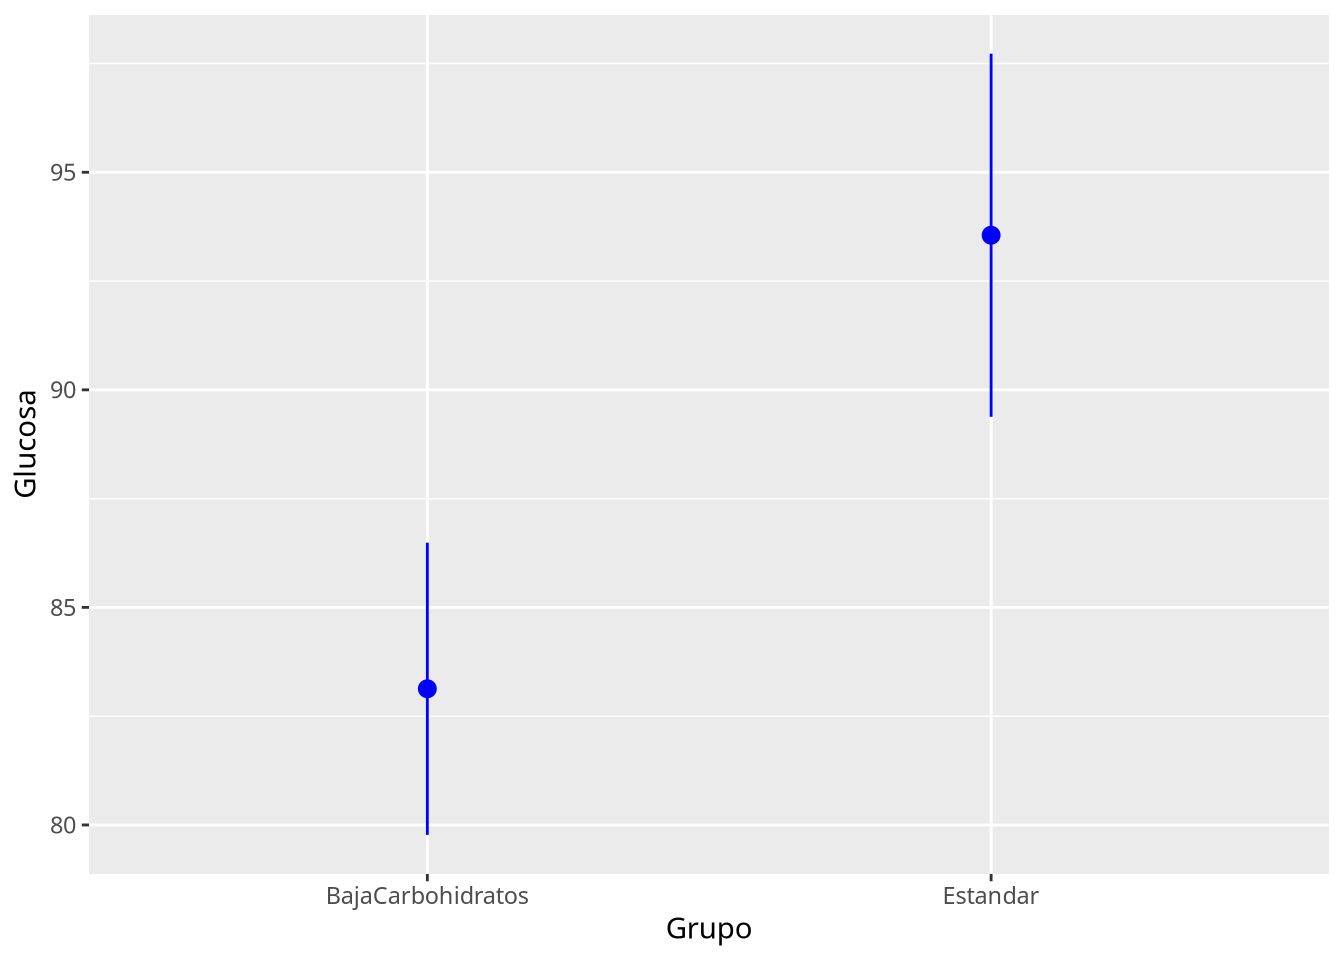
\includegraphics[keepaspectratio]{01-contrastes-parametricos-practicas_files/figure-pdf/unnamed-chunk-15-1.pdf}}

\end{tcolorbox}

\begin{exercise}[]\protect\hypertarget{exr-contraste-comparacion-medias-expresion-genica}{}\label{exr-contraste-comparacion-medias-expresion-genica}

Se ha realizado un estudio para comparar los niveles de expresión de un
gen en función de la dieta (vegetariana u omnívora). Los datos del
estudio están en el fichero
\href{datos/expresion-genica-dietas.csv}{expresion-genica-dietas.csv}.
Realizar el contraste de hipótesis adecuado para comparar las medias de
los dos grupos.

\end{exercise}

\begin{tcolorbox}[enhanced jigsaw, breakable, opacityback=0, colbacktitle=quarto-callout-tip-color!10!white, colframe=quarto-callout-tip-color-frame, left=2mm, titlerule=0mm, coltitle=black, colback=white, bottomtitle=1mm, toptitle=1mm, opacitybacktitle=0.6, title=\textcolor{quarto-callout-tip-color}{\faLightbulb}\hspace{0.5em}{Solución}, leftrule=.75mm, bottomrule=.15mm, toprule=.15mm, rightrule=.15mm, arc=.35mm]

En primer lugar cargamos los datos en un data frame y mostramos las
primeras filas.

\begin{Shaded}
\begin{Highlighting}[]
\FunctionTok{library}\NormalTok{(tidyverse)}
\FunctionTok{library}\NormalTok{(knitr)}
\FunctionTok{library}\NormalTok{(broom)}
\NormalTok{df }\OtherTok{\textless{}{-}} \FunctionTok{read.csv}\NormalTok{(}\StringTok{"datos/expresion{-}genica{-}dietas.csv"}\NormalTok{)}
\FunctionTok{head}\NormalTok{(df)}
\end{Highlighting}
\end{Shaded}

\begin{verbatim}
        Grupo Expresion.Genica
1 Vegetariana            0.735
2 Vegetariana            1.221
3 Vegetariana            0.881
4 Vegetariana            1.342
5 Vegetariana            0.924
6 Vegetariana            1.665
\end{verbatim}

Hacemos un análisis descriptivo básico.

\begin{Shaded}
\begin{Highlighting}[]
\NormalTok{df }\SpecialCharTok{|\textgreater{}} 
    \FunctionTok{group\_by}\NormalTok{(Grupo) }\SpecialCharTok{|\textgreater{}} 
    \FunctionTok{summarise}\NormalTok{(}
        \AttributeTok{n =} \FunctionTok{n}\NormalTok{(),}
        \AttributeTok{media =} \FunctionTok{mean}\NormalTok{(Expresion.Genica, }\AttributeTok{na.rm =} \ConstantTok{TRUE}\NormalTok{),}
\NormalTok{        desviación\_típica }\OtherTok{=} \FunctionTok{sd}\NormalTok{(Expresion.Genica, }\AttributeTok{na.rm =} \ConstantTok{TRUE}\NormalTok{)}
\NormalTok{    ) }\SpecialCharTok{|\textgreater{}} 
    \FunctionTok{kable}\NormalTok{()}
\end{Highlighting}
\end{Shaded}

\begin{longtable}[]{@{}lrrr@{}}
\toprule\noalign{}
Grupo & n & media & desviación\_típica \\
\midrule\noalign{}
\endhead
\bottomrule\noalign{}
\endlastfoot
Omnivora & 25 & 1.62672 & 0.4087498 \\
Vegetariana & 20 & 1.14680 & 0.2917002 \\
\end{longtable}

Comprobamos la normalidad de los datos.

\begin{Shaded}
\begin{Highlighting}[]
\NormalTok{df }\SpecialCharTok{|\textgreater{}} 
    \FunctionTok{group\_by}\NormalTok{(Grupo) }\SpecialCharTok{|\textgreater{}} 
    \FunctionTok{summarise}\NormalTok{(}\AttributeTok{test =} \FunctionTok{tidy}\NormalTok{(}\FunctionTok{shapiro.test}\NormalTok{(Expresion.Genica))) }\SpecialCharTok{|\textgreater{}} 
    \FunctionTok{unnest}\NormalTok{(test) }\SpecialCharTok{|\textgreater{}} 
    \FunctionTok{kable}\NormalTok{()}
\end{Highlighting}
\end{Shaded}

\begin{longtable}[]{@{}lrrl@{}}
\toprule\noalign{}
Grupo & statistic & p.value & method \\
\midrule\noalign{}
\endhead
\bottomrule\noalign{}
\endlastfoot
Omnivora & 0.9578432 & 0.3731950 & Shapiro-Wilk normality test \\
Vegetariana & 0.9372700 & 0.2128177 & Shapiro-Wilk normality test \\
\end{longtable}

Como el p-valor es mayor que el nivel de significación 0.05 en ambos
grupos aceptamos la hipótesis de normalidad.

A continuación aplicamos el contraste de comparación de varianzas de
poblaciones normales.

\begin{Shaded}
\begin{Highlighting}[]
\FunctionTok{tidy}\NormalTok{(}\FunctionTok{var.test}\NormalTok{ (Expresion.Genica }\SpecialCharTok{\textasciitilde{}}\NormalTok{ Grupo, }\AttributeTok{data =}\NormalTok{ df)) }\SpecialCharTok{|\textgreater{}} 
    \FunctionTok{kable}\NormalTok{()}
\end{Highlighting}
\end{Shaded}

\begin{verbatim}
Multiple parameters; naming those columns num.df, den.df
\end{verbatim}

\begin{longtable}[]{@{}
  >{\raggedleft\arraybackslash}p{(\linewidth - 16\tabcolsep) * \real{0.0841}}
  >{\raggedleft\arraybackslash}p{(\linewidth - 16\tabcolsep) * \real{0.0654}}
  >{\raggedleft\arraybackslash}p{(\linewidth - 16\tabcolsep) * \real{0.0654}}
  >{\raggedleft\arraybackslash}p{(\linewidth - 16\tabcolsep) * \real{0.0935}}
  >{\raggedleft\arraybackslash}p{(\linewidth - 16\tabcolsep) * \real{0.0935}}
  >{\raggedleft\arraybackslash}p{(\linewidth - 16\tabcolsep) * \real{0.0935}}
  >{\raggedleft\arraybackslash}p{(\linewidth - 16\tabcolsep) * \real{0.0935}}
  >{\raggedright\arraybackslash}p{(\linewidth - 16\tabcolsep) * \real{0.2991}}
  >{\raggedright\arraybackslash}p{(\linewidth - 16\tabcolsep) * \real{0.1121}}@{}}
\toprule\noalign{}
\begin{minipage}[b]{\linewidth}\raggedleft
estimate
\end{minipage} & \begin{minipage}[b]{\linewidth}\raggedleft
num.df
\end{minipage} & \begin{minipage}[b]{\linewidth}\raggedleft
den.df
\end{minipage} & \begin{minipage}[b]{\linewidth}\raggedleft
statistic
\end{minipage} & \begin{minipage}[b]{\linewidth}\raggedleft
p.value
\end{minipage} & \begin{minipage}[b]{\linewidth}\raggedleft
conf.low
\end{minipage} & \begin{minipage}[b]{\linewidth}\raggedleft
conf.high
\end{minipage} & \begin{minipage}[b]{\linewidth}\raggedright
method
\end{minipage} & \begin{minipage}[b]{\linewidth}\raggedright
alternative
\end{minipage} \\
\midrule\noalign{}
\endhead
\bottomrule\noalign{}
\endlastfoot
1.963548 & 24 & 19 & 1.963548 & 0.1373252 & 0.8006898 & 4.604823 & F
test to compare two variances & two.sided \\
\end{longtable}

Como el p-valor es mayor que el nivel de significación \(0.05\) asumimos
varianzas iguales.

Finalmente aplicamos el contraste t para la comparación de medias de dos
poblaciones independientes con varianzas iguales.

\begin{Shaded}
\begin{Highlighting}[]
\FunctionTok{tidy}\NormalTok{(}\FunctionTok{t.test}\NormalTok{(Expresion.Genica }\SpecialCharTok{\textasciitilde{}}\NormalTok{ Grupo, }\AttributeTok{data =}\NormalTok{ df, }\AttributeTok{alternative =} \StringTok{"two.sided"}\NormalTok{, }\AttributeTok{var.equal =} \ConstantTok{TRUE}\NormalTok{), }\AttributeTok{conf.int =} \ConstantTok{TRUE}\NormalTok{) }\SpecialCharTok{|\textgreater{}} 
    \FunctionTok{kable}\NormalTok{()}
\end{Highlighting}
\end{Shaded}

\begin{longtable}[]{@{}
  >{\raggedleft\arraybackslash}p{(\linewidth - 18\tabcolsep) * \real{0.0833}}
  >{\raggedleft\arraybackslash}p{(\linewidth - 18\tabcolsep) * \real{0.0926}}
  >{\raggedleft\arraybackslash}p{(\linewidth - 18\tabcolsep) * \real{0.0926}}
  >{\raggedleft\arraybackslash}p{(\linewidth - 18\tabcolsep) * \real{0.0926}}
  >{\raggedleft\arraybackslash}p{(\linewidth - 18\tabcolsep) * \real{0.0833}}
  >{\raggedleft\arraybackslash}p{(\linewidth - 18\tabcolsep) * \real{0.0926}}
  >{\raggedleft\arraybackslash}p{(\linewidth - 18\tabcolsep) * \real{0.0926}}
  >{\raggedleft\arraybackslash}p{(\linewidth - 18\tabcolsep) * \real{0.0926}}
  >{\raggedright\arraybackslash}p{(\linewidth - 18\tabcolsep) * \real{0.1667}}
  >{\raggedright\arraybackslash}p{(\linewidth - 18\tabcolsep) * \real{0.1111}}@{}}
\toprule\noalign{}
\begin{minipage}[b]{\linewidth}\raggedleft
estimate
\end{minipage} & \begin{minipage}[b]{\linewidth}\raggedleft
estimate1
\end{minipage} & \begin{minipage}[b]{\linewidth}\raggedleft
estimate2
\end{minipage} & \begin{minipage}[b]{\linewidth}\raggedleft
statistic
\end{minipage} & \begin{minipage}[b]{\linewidth}\raggedleft
p.value
\end{minipage} & \begin{minipage}[b]{\linewidth}\raggedleft
parameter
\end{minipage} & \begin{minipage}[b]{\linewidth}\raggedleft
conf.low
\end{minipage} & \begin{minipage}[b]{\linewidth}\raggedleft
conf.high
\end{minipage} & \begin{minipage}[b]{\linewidth}\raggedright
method
\end{minipage} & \begin{minipage}[b]{\linewidth}\raggedright
alternative
\end{minipage} \\
\midrule\noalign{}
\endhead
\bottomrule\noalign{}
\endlastfoot
0.47992 & 1.62672 & 1.1468 & 4.422438 & 6.54e-05 & 43 & 0.2610699 &
0.6987701 & Two Sample t-test & two.sided \\
\end{longtable}

Como el p-valor es menor que el nivel de significación \(0.05\)
rechazamos la hipótesis nula y concluimos que existen diferencias
estadísticamente significativas entre el nivel medio de expresión génica
de las dos dietas. Además, según el intervalo de confianza del 95\%, el
nivel de expresión génica con la dieta omnívora estaría sería entre
\(0.261\) y \(0.699\) mayor que con la dieta vegetariana.

\end{tcolorbox}

\begin{exercise}[]\protect\hypertarget{exr-contraste-comparacion-proporciones-vitamina-c}{}\label{exr-contraste-comparacion-proporciones-vitamina-c}

Se utiliza un grupo de 150 pacientes para comprobar la teoría de que la
vitamina C tiene alguna influencia en el tratamiento del cáncer. Los 150
pacientes fueron divididos en dos grupos de 75. Un grupo recibió 10
gramos de vitamina C y el otro un placebo cada día, además de la
medicación habitual. De los que recibieron la vitamina C, 47 presentaban
alguna mejoría al cabo de cuatro semanas, mientras que de los que
recibieron el placebo, 43 experimentaron mejoría. Contrastar la
hipótesis de que la vitamina C tiene influencia en el tratamiento del
cáncer con un nivel de significación del 5\%.

\end{exercise}

\begin{tcolorbox}[enhanced jigsaw, breakable, opacityback=0, colbacktitle=quarto-callout-tip-color!10!white, colframe=quarto-callout-tip-color-frame, left=2mm, titlerule=0mm, coltitle=black, colback=white, bottomtitle=1mm, toptitle=1mm, opacitybacktitle=0.6, title=\textcolor{quarto-callout-tip-color}{\faLightbulb}\hspace{0.5em}{Solución}, leftrule=.75mm, bottomrule=.15mm, toprule=.15mm, rightrule=.15mm, arc=.35mm]

\begin{Shaded}
\begin{Highlighting}[]
\FunctionTok{tidy}\NormalTok{(}\FunctionTok{prop.test}\NormalTok{(}\FunctionTok{c}\NormalTok{(}\DecValTok{47}\NormalTok{, }\DecValTok{43}\NormalTok{), }\FunctionTok{c}\NormalTok{(}\DecValTok{75}\NormalTok{, }\DecValTok{75}\NormalTok{), }\AttributeTok{alternative =} \StringTok{"two.sided"}\NormalTok{)) }\SpecialCharTok{|\textgreater{}} 
    \FunctionTok{kable}\NormalTok{()}
\end{Highlighting}
\end{Shaded}

\begin{longtable}[]{@{}
  >{\raggedleft\arraybackslash}p{(\linewidth - 16\tabcolsep) * \real{0.0658}}
  >{\raggedleft\arraybackslash}p{(\linewidth - 16\tabcolsep) * \real{0.0658}}
  >{\raggedleft\arraybackslash}p{(\linewidth - 16\tabcolsep) * \real{0.0658}}
  >{\raggedleft\arraybackslash}p{(\linewidth - 16\tabcolsep) * \real{0.0658}}
  >{\raggedleft\arraybackslash}p{(\linewidth - 16\tabcolsep) * \real{0.0658}}
  >{\raggedleft\arraybackslash}p{(\linewidth - 16\tabcolsep) * \real{0.0724}}
  >{\raggedleft\arraybackslash}p{(\linewidth - 16\tabcolsep) * \real{0.0658}}
  >{\raggedright\arraybackslash}p{(\linewidth - 16\tabcolsep) * \real{0.4539}}
  >{\raggedright\arraybackslash}p{(\linewidth - 16\tabcolsep) * \real{0.0789}}@{}}
\toprule\noalign{}
\begin{minipage}[b]{\linewidth}\raggedleft
estimate1
\end{minipage} & \begin{minipage}[b]{\linewidth}\raggedleft
estimate2
\end{minipage} & \begin{minipage}[b]{\linewidth}\raggedleft
statistic
\end{minipage} & \begin{minipage}[b]{\linewidth}\raggedleft
p.value
\end{minipage} & \begin{minipage}[b]{\linewidth}\raggedleft
parameter
\end{minipage} & \begin{minipage}[b]{\linewidth}\raggedleft
conf.low
\end{minipage} & \begin{minipage}[b]{\linewidth}\raggedleft
conf.high
\end{minipage} & \begin{minipage}[b]{\linewidth}\raggedright
method
\end{minipage} & \begin{minipage}[b]{\linewidth}\raggedright
alternative
\end{minipage} \\
\midrule\noalign{}
\endhead
\bottomrule\noalign{}
\endlastfoot
0.6266667 & 0.5733333 & 0.25 & 0.6170751 & 1 & -0.1165647 & 0.2232313 &
2-sample test for equality of proportions with continuity correction &
two.sided \\
\end{longtable}

Como el p-valor del contraste es mayor que el nivel de significación
\(0.05\), se acepta la hipótesis nula y se concluye que no hay
evidencias significativas de que la vitamina C influya en el tratamiento
del cáncer.

\end{tcolorbox}

\begin{exercise}[]\protect\hypertarget{exr-contraste-proporcion-consumo-alcohol}{}\label{exr-contraste-proporcion-consumo-alcohol}

En un estudio sobre el consumo de alcohol entre los jóvenes durante los
fines de semana, se preguntó a 100 chicos y a 125 chicas, de los que 63
chicos y 59 chicas contestaron que consumían. En vista de estos datos,
¿existe alguna diferencia significativa entre las proporciones de chicos
y chicas que consumen alcohol los fines de semana?

\end{exercise}

\begin{tcolorbox}[enhanced jigsaw, breakable, opacityback=0, colbacktitle=quarto-callout-tip-color!10!white, colframe=quarto-callout-tip-color-frame, left=2mm, titlerule=0mm, coltitle=black, colback=white, bottomtitle=1mm, toptitle=1mm, opacitybacktitle=0.6, title=\textcolor{quarto-callout-tip-color}{\faLightbulb}\hspace{0.5em}{Solución}, leftrule=.75mm, bottomrule=.15mm, toprule=.15mm, rightrule=.15mm, arc=.35mm]

\begin{Shaded}
\begin{Highlighting}[]
\FunctionTok{tidy}\NormalTok{(}\FunctionTok{prop.test}\NormalTok{(}\FunctionTok{c}\NormalTok{(}\DecValTok{63}\NormalTok{, }\DecValTok{59}\NormalTok{), }\FunctionTok{c}\NormalTok{(}\DecValTok{100}\NormalTok{, }\DecValTok{125}\NormalTok{), }\AttributeTok{alternative =} \StringTok{"two.sided"}\NormalTok{), }\AttributeTok{conf.int =} \ConstantTok{TRUE}\NormalTok{) }\SpecialCharTok{|\textgreater{}} 
    \FunctionTok{kable}\NormalTok{()}
\end{Highlighting}
\end{Shaded}

\begin{longtable}[]{@{}
  >{\raggedleft\arraybackslash}p{(\linewidth - 16\tabcolsep) * \real{0.0662}}
  >{\raggedleft\arraybackslash}p{(\linewidth - 16\tabcolsep) * \real{0.0662}}
  >{\raggedleft\arraybackslash}p{(\linewidth - 16\tabcolsep) * \real{0.0662}}
  >{\raggedleft\arraybackslash}p{(\linewidth - 16\tabcolsep) * \real{0.0662}}
  >{\raggedleft\arraybackslash}p{(\linewidth - 16\tabcolsep) * \real{0.0662}}
  >{\raggedleft\arraybackslash}p{(\linewidth - 16\tabcolsep) * \real{0.0662}}
  >{\raggedleft\arraybackslash}p{(\linewidth - 16\tabcolsep) * \real{0.0662}}
  >{\raggedright\arraybackslash}p{(\linewidth - 16\tabcolsep) * \real{0.4570}}
  >{\raggedright\arraybackslash}p{(\linewidth - 16\tabcolsep) * \real{0.0795}}@{}}
\toprule\noalign{}
\begin{minipage}[b]{\linewidth}\raggedleft
estimate1
\end{minipage} & \begin{minipage}[b]{\linewidth}\raggedleft
estimate2
\end{minipage} & \begin{minipage}[b]{\linewidth}\raggedleft
statistic
\end{minipage} & \begin{minipage}[b]{\linewidth}\raggedleft
p.value
\end{minipage} & \begin{minipage}[b]{\linewidth}\raggedleft
parameter
\end{minipage} & \begin{minipage}[b]{\linewidth}\raggedleft
conf.low
\end{minipage} & \begin{minipage}[b]{\linewidth}\raggedleft
conf.high
\end{minipage} & \begin{minipage}[b]{\linewidth}\raggedright
method
\end{minipage} & \begin{minipage}[b]{\linewidth}\raggedright
alternative
\end{minipage} \\
\midrule\noalign{}
\endhead
\bottomrule\noalign{}
\endlastfoot
0.63 & 0.472 & 4.968989 & 0.0258057 & 1 & 0.0201075 & 0.2958925 &
2-sample test for equality of proportions with continuity correction &
two.sided \\
\end{longtable}

Como el p-valor del contraste es menor que el nivel de significación
\(0.05\), se rechaza la hipótesis nula y se concluye que hay diferencias
estadísticamente significativas entre la proporción de chicos y chicas
que consumen alcohol los fines de semana. Además, según el intervalo de
confianza del 95\%, el porcentaje de chicos sería entre un \(2.01\)\% y
un \(29.6\)\% mayor que el de chicas.

\end{tcolorbox}

\begin{exercise}[]\protect\hypertarget{exr-contraste-anova-suplementacion}{}\label{exr-contraste-anova-suplementacion}

En un estudio de genómica nutricional, se evalúa cómo afecta la
suplementación con diferentes tipos de macronutrientes a la expresión de
un gen relacionado con el metabolismo energético. Los investigadores
dividen a los participantes en tres grupos, cada uno recibiendo una
dieta suplementada (1 carbohidratos, 2 proteínas y 3 grasas).Se mide el
nivel de expresión génica (ΔCt, relativo a un gen de referencia) en 25
individuos por grupo. Los resultados se recogen en el fichero
\href{datos/expresion-genica-suplementacion.csv}{expresion-genica-suplementacion.csv}.
Realizar el contraste de hipótesis adecuado para comparar ver si hay
diferencias estadísticamente significativas entre las expresiones
génicas de los tres grupos.

\end{exercise}

\begin{tcolorbox}[enhanced jigsaw, breakable, opacityback=0, colbacktitle=quarto-callout-tip-color!10!white, colframe=quarto-callout-tip-color-frame, left=2mm, titlerule=0mm, coltitle=black, colback=white, bottomtitle=1mm, toptitle=1mm, opacitybacktitle=0.6, title=\textcolor{quarto-callout-tip-color}{\faLightbulb}\hspace{0.5em}{Solución}, leftrule=.75mm, bottomrule=.15mm, toprule=.15mm, rightrule=.15mm, arc=.35mm]

En primer lugar cargamos los datos en un data frame y mostramos las
primeras filas.

\begin{Shaded}
\begin{Highlighting}[]
\FunctionTok{library}\NormalTok{(tidyverse)}
\FunctionTok{library}\NormalTok{(knitr)}
\FunctionTok{library}\NormalTok{(broom)}
\NormalTok{df }\OtherTok{\textless{}{-}} \FunctionTok{read.csv}\NormalTok{(}\StringTok{"datos/expresion{-}genica{-}suplementacion.csv"}\NormalTok{)}
\FunctionTok{head}\NormalTok{(df)}
\end{Highlighting}
\end{Shaded}

\begin{verbatim}
  Suplementacion Expresion.genica
1  Carbohidratos            1.299
2  Carbohidratos            1.172
3  Carbohidratos            1.330
4  Carbohidratos            1.505
5  Carbohidratos            1.153
6  Carbohidratos            1.153
\end{verbatim}

Hacemos un análisis descriptivo básico.

\begin{Shaded}
\begin{Highlighting}[]
\NormalTok{df }\SpecialCharTok{|\textgreater{}} 
    \FunctionTok{group\_by}\NormalTok{(Suplementacion) }\SpecialCharTok{|\textgreater{}} 
    \FunctionTok{summarise}\NormalTok{(}
        \AttributeTok{n =} \FunctionTok{n}\NormalTok{(),}
        \AttributeTok{media =} \FunctionTok{mean}\NormalTok{(Expresion.genica, }\AttributeTok{na.rm =} \ConstantTok{TRUE}\NormalTok{),}
\NormalTok{        desviación\_típica }\OtherTok{=} \FunctionTok{sd}\NormalTok{(Expresion.genica, }\AttributeTok{na.rm =} \ConstantTok{TRUE}\NormalTok{)}
\NormalTok{    ) }\SpecialCharTok{|\textgreater{}} 
    \FunctionTok{kable}\NormalTok{()}
\end{Highlighting}
\end{Shaded}

\begin{longtable}[]{@{}lrrr@{}}
\toprule\noalign{}
Suplementacion & n & media & desviación\_típica \\
\midrule\noalign{}
\endhead
\bottomrule\noalign{}
\endlastfoot
Carbohidratos & 25 & 1.16728 & 0.1913774 \\
Grasas & 25 & 1.42656 & 0.2468005 \\
Proteinas & 25 & 1.41380 & 0.2777301 \\
\end{longtable}

Aplicamos el contraste de ANOVA para la comparación de medias de más de
dos poblaciones independientes.

\begin{Shaded}
\begin{Highlighting}[]
\NormalTok{anova }\OtherTok{\textless{}{-}} \FunctionTok{aov}\NormalTok{(Expresion.genica }\SpecialCharTok{\textasciitilde{}}\NormalTok{ Suplementacion, }\AttributeTok{data =}\NormalTok{ df)}
\FunctionTok{tidy}\NormalTok{(anova) }\SpecialCharTok{|\textgreater{}} 
    \FunctionTok{kable}\NormalTok{()}
\end{Highlighting}
\end{Shaded}

\begin{longtable}[]{@{}lrrrrr@{}}
\toprule\noalign{}
term & df & sumsq & meansq & statistic & p.value \\
\midrule\noalign{}
\endhead
\bottomrule\noalign{}
\endlastfoot
Suplementacion & 2 & 1.068009 & 0.5340044 & 9.171666 & 0.000283 \\
Residuals & 72 & 4.192075 & 0.0582233 & NA & NA \\
\end{longtable}

Como el p-valor es menor que el nivel de significación \(0.05\),
rechazamos la hipótesis nula y concluimos que existen pruebas
estadísticamente significativas de que el nivel de expresión génica
depende del la dieta.

A continuación comprobamos si se cumplen los requisitos del contraste de
ANOVA.

\begin{enumerate}
\def\labelenumi{\alph{enumi}.}
\item
  Normalidad de los residuos.

\begin{Shaded}
\begin{Highlighting}[]
\NormalTok{residuals }\OtherTok{\textless{}{-}} \FunctionTok{residuals}\NormalTok{(anova)}
\FunctionTok{par}\NormalTok{(}\AttributeTok{mfrow =} \FunctionTok{c}\NormalTok{(}\DecValTok{1}\NormalTok{, }\DecValTok{2}\NormalTok{))  }
\FunctionTok{hist}\NormalTok{(residuals)}
\FunctionTok{qqnorm}\NormalTok{(residuals, }\AttributeTok{main =} \StringTok{"Q{-}Q Plot of Residuals"}\NormalTok{)}
\FunctionTok{qqline}\NormalTok{(residuals, }\AttributeTok{col =} \StringTok{"red"}\NormalTok{, }\AttributeTok{lwd =} \DecValTok{2}\NormalTok{)}
\end{Highlighting}
\end{Shaded}

  \pandocbounded{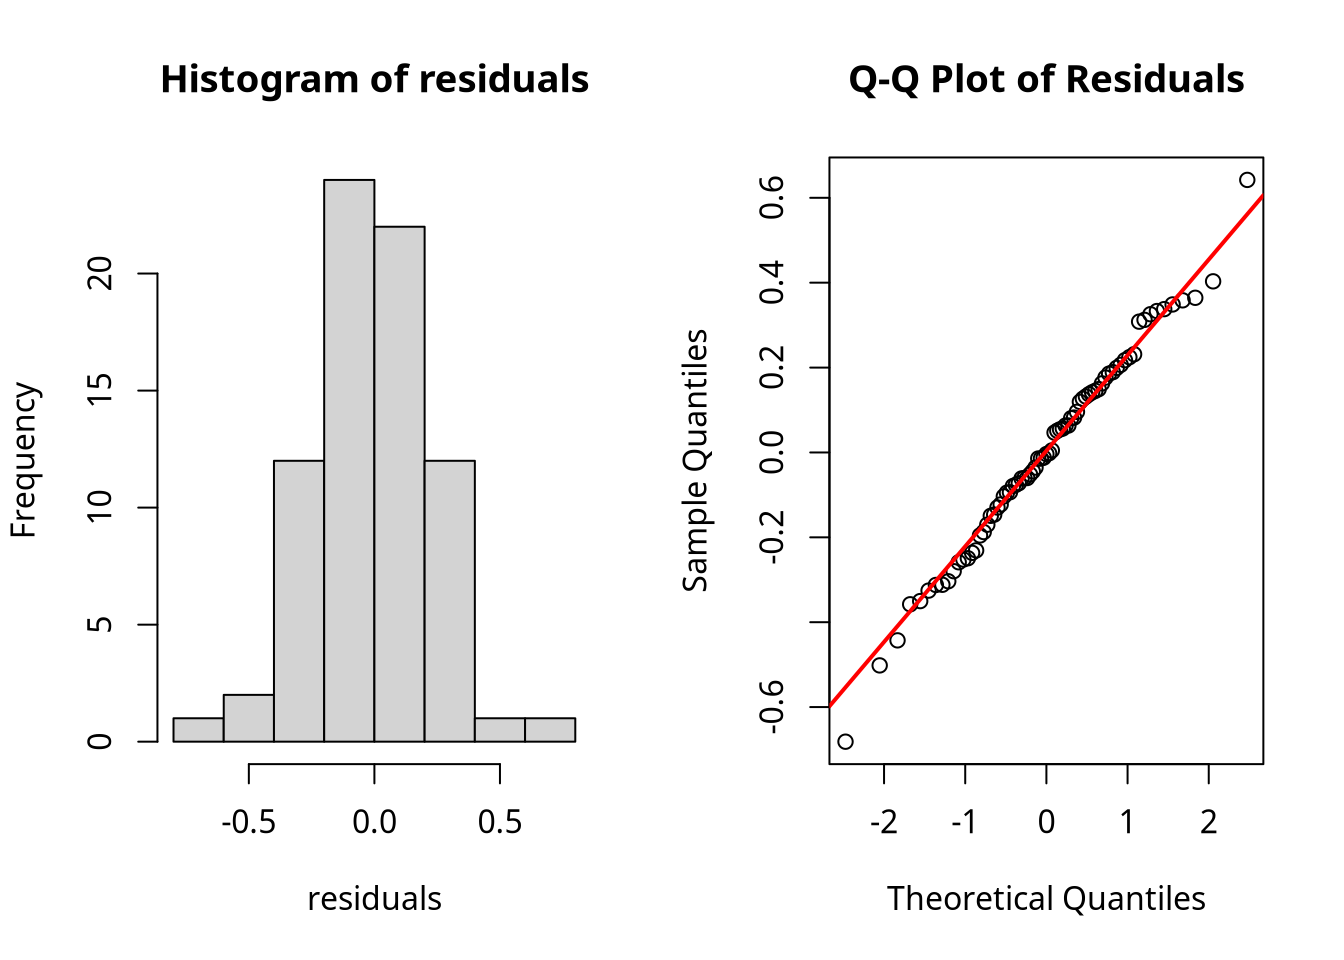
\includegraphics[keepaspectratio]{01-contrastes-parametricos-practicas_files/figure-pdf/unnamed-chunk-26-1.pdf}}

\begin{Shaded}
\begin{Highlighting}[]
\FunctionTok{tidy}\NormalTok{(}\FunctionTok{shapiro.test}\NormalTok{(residuals)) }\SpecialCharTok{|\textgreater{}} 
\FunctionTok{kable}\NormalTok{()}
\end{Highlighting}
\end{Shaded}

  \begin{longtable}[]{@{}rrl@{}}
  \toprule\noalign{}
  statistic & p.value & method \\
  \midrule\noalign{}
  \endhead
  \bottomrule\noalign{}
  \endlastfoot
  0.9926311 & 0.9455761 & Shapiro-Wilk normality test \\
  \end{longtable}

  Tanto el histograma como el gráfico de cuantiles no muestran una
  desviación significativa de una distribución normal, y como el p-valor
  del contraste de normalidad es mayor que el nivel de significación
  \(0.05\), se asume que los residuos siguen una distribución normal.
\item
  Homogeneidad de varianzas. Aplicamos el test de Levene para la
  comparación de varianzas.

\begin{Shaded}
\begin{Highlighting}[]
\FunctionTok{library}\NormalTok{(car)}
\end{Highlighting}
\end{Shaded}

\begin{verbatim}
Cargando paquete requerido: carData
\end{verbatim}

\begin{verbatim}

Adjuntando el paquete: 'car'
\end{verbatim}

\begin{verbatim}
The following object is masked from 'package:dplyr':

    recode
\end{verbatim}

\begin{verbatim}
The following object is masked from 'package:purrr':

    some
\end{verbatim}

\begin{Shaded}
\begin{Highlighting}[]
\FunctionTok{tidy}\NormalTok{(}\FunctionTok{leveneTest}\NormalTok{(Expresion.genica }\SpecialCharTok{\textasciitilde{}}\NormalTok{ Suplementacion, }\AttributeTok{data =}\NormalTok{ df)) }\SpecialCharTok{|\textgreater{}} 
\FunctionTok{kable}\NormalTok{()}
\end{Highlighting}
\end{Shaded}

\begin{verbatim}
Warning in leveneTest.default(y = y, group = group, ...): group coerced to
factor.
\end{verbatim}

  \begin{longtable}[]{@{}rrrr@{}}
  \toprule\noalign{}
  statistic & p.value & df & df.residual \\
  \midrule\noalign{}
  \endhead
  \bottomrule\noalign{}
  \endlastfoot
  1.582187 & 0.2125867 & 2 & 72 \\
  \end{longtable}

  Como el p-valor es mayor que el nivel de significación \(0.05\) se
  acepta la hipótesis nula y se asume homogeneidad de varianzas.

  Así pues, se cumplen los requisitos para el contraste de ANOVA.
\end{enumerate}

Finalmente hacemos una comparación de medias por pares para ver entre
qué grupos hay diferencias estadísticamente significativas.

\begin{Shaded}
\begin{Highlighting}[]
\FunctionTok{tidy}\NormalTok{(}\FunctionTok{TukeyHSD}\NormalTok{(anova)) }\SpecialCharTok{|\textgreater{}} 
    \FunctionTok{kable}\NormalTok{()}
\end{Highlighting}
\end{Shaded}

\begin{longtable}[]{@{}
  >{\raggedright\arraybackslash}p{(\linewidth - 12\tabcolsep) * \real{0.1630}}
  >{\raggedright\arraybackslash}p{(\linewidth - 12\tabcolsep) * \real{0.2609}}
  >{\raggedleft\arraybackslash}p{(\linewidth - 12\tabcolsep) * \real{0.1196}}
  >{\raggedleft\arraybackslash}p{(\linewidth - 12\tabcolsep) * \real{0.0978}}
  >{\raggedleft\arraybackslash}p{(\linewidth - 12\tabcolsep) * \real{0.1196}}
  >{\raggedleft\arraybackslash}p{(\linewidth - 12\tabcolsep) * \real{0.1087}}
  >{\raggedleft\arraybackslash}p{(\linewidth - 12\tabcolsep) * \real{0.1304}}@{}}
\toprule\noalign{}
\begin{minipage}[b]{\linewidth}\raggedright
term
\end{minipage} & \begin{minipage}[b]{\linewidth}\raggedright
contrast
\end{minipage} & \begin{minipage}[b]{\linewidth}\raggedleft
null.value
\end{minipage} & \begin{minipage}[b]{\linewidth}\raggedleft
estimate
\end{minipage} & \begin{minipage}[b]{\linewidth}\raggedleft
conf.low
\end{minipage} & \begin{minipage}[b]{\linewidth}\raggedleft
conf.high
\end{minipage} & \begin{minipage}[b]{\linewidth}\raggedleft
adj.p.value
\end{minipage} \\
\midrule\noalign{}
\endhead
\bottomrule\noalign{}
\endlastfoot
Suplementacion & Grasas-Carbohidratos & 0 & 0.25928 & 0.0959528 &
0.4226072 & 0.0008694 \\
Suplementacion & Proteinas-Carbohidratos & 0 & 0.24652 & 0.0831928 &
0.4098472 & 0.0016018 \\
Suplementacion & Proteinas-Grasas & 0 & -0.01276 & -0.1760872 &
0.1505672 & 0.9809191 \\
\end{longtable}

Se observan diferencias estadísticamente significativas entre las medias
de la dieta basada en grasas y la basada en carbohidratos (p-valor
\(0.0008 < 0.05\)) y también entre la dieta basada en proteínas y la
basada en carbohidratos (p-valor \(0.0016 < 0.05\)), pero no entre la
dieta basada en proteínas y la basada en grasas (p-valor
\(0.981 > 0.05\)).

\begin{Shaded}
\begin{Highlighting}[]
\FunctionTok{tidy}\NormalTok{(}\FunctionTok{TukeyHSD}\NormalTok{(anova)) }\SpecialCharTok{|\textgreater{}} 
    \FunctionTok{ggplot}\NormalTok{(}\FunctionTok{aes}\NormalTok{(}\AttributeTok{x =}\NormalTok{ contrast, }\AttributeTok{y =}\NormalTok{ estimate)) }\SpecialCharTok{+}
    \FunctionTok{geom\_errorbar}\NormalTok{(}\FunctionTok{aes}\NormalTok{(}\AttributeTok{ymin =}\NormalTok{ conf.low, }\AttributeTok{ymax =}\NormalTok{ conf.high), }\AttributeTok{width =} \FloatTok{0.2}\NormalTok{, }\AttributeTok{color =} \StringTok{"blue"}\NormalTok{) }\SpecialCharTok{+}
    \FunctionTok{geom\_point}\NormalTok{(}\AttributeTok{size =} \DecValTok{3}\NormalTok{, }\AttributeTok{color =} \StringTok{"red"}\NormalTok{) }\SpecialCharTok{+}
    \FunctionTok{geom\_hline}\NormalTok{(}\AttributeTok{yintercept =} \DecValTok{0}\NormalTok{, }\AttributeTok{linetype =} \StringTok{"dashed"}\NormalTok{)}
\end{Highlighting}
\end{Shaded}

\pandocbounded{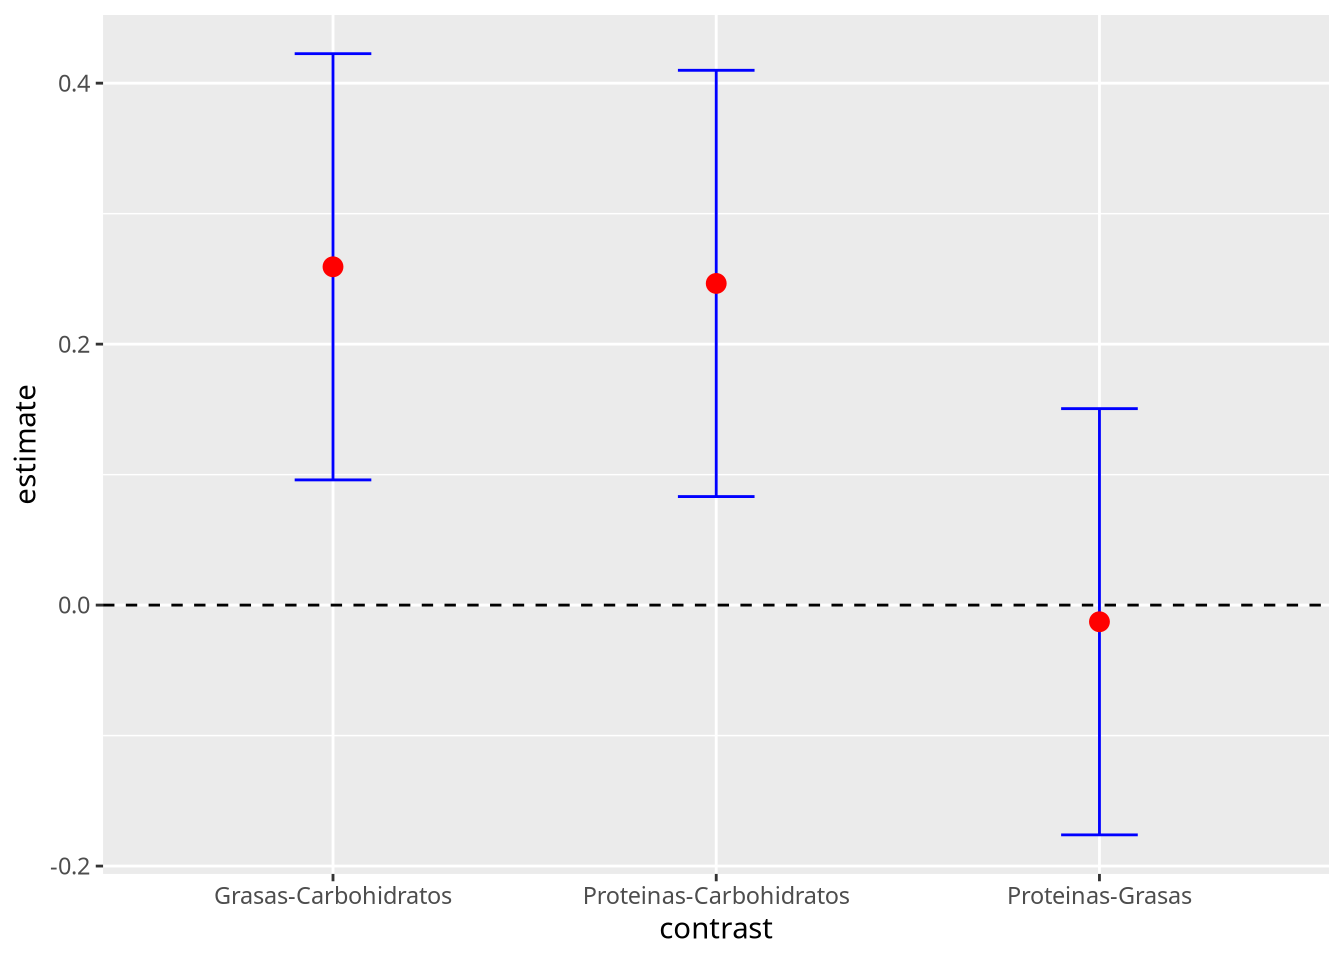
\includegraphics[keepaspectratio]{01-contrastes-parametricos-practicas_files/figure-pdf/unnamed-chunk-29-1.pdf}}

\end{tcolorbox}

\begin{exercise}[]\protect\hypertarget{exr-contraste-anova-interaccion-dieta-farmaco}{}\label{exr-contraste-anova-interaccion-dieta-farmaco}

En un estudio diseñado para analizar la influencia de un tipo de dieta y
de un fármaco en el peso corporal perdido, se ha anotado el número de Kg
perdidos en un grupo de personas al cabo de 3 meses de dieta y de tomar
el fármaco en el fichero
\href{datos/interaccion-dieta-farmaco.csv}{interaccion-dieta-farmaco.csv}.
Realizar el contraste de hipótesis adecuado para ver si el peso perdido
depende de la dieta, del fármaco y de la interacción entre ambos.

\end{exercise}

\begin{tcolorbox}[enhanced jigsaw, breakable, opacityback=0, colbacktitle=quarto-callout-tip-color!10!white, colframe=quarto-callout-tip-color-frame, left=2mm, titlerule=0mm, coltitle=black, colback=white, bottomtitle=1mm, toptitle=1mm, opacitybacktitle=0.6, title=\textcolor{quarto-callout-tip-color}{\faLightbulb}\hspace{0.5em}{Solución}, leftrule=.75mm, bottomrule=.15mm, toprule=.15mm, rightrule=.15mm, arc=.35mm]

En primer lugar cargamos los datos en un data frame y mostramos las
primeras filas.

\begin{Shaded}
\begin{Highlighting}[]
\FunctionTok{library}\NormalTok{(tidyverse)}
\FunctionTok{library}\NormalTok{(knitr)}
\FunctionTok{library}\NormalTok{(broom)}
\NormalTok{df }\OtherTok{\textless{}{-}} \FunctionTok{read.csv}\NormalTok{(}\StringTok{"datos/interaccion{-}dieta{-}farmaco.csv"}\NormalTok{)}
\FunctionTok{head}\NormalTok{(df)}
\end{Highlighting}
\end{Shaded}

\begin{verbatim}
  Dieta Farmaco Perdida_peso
1    No      No          1.5
2    No      No          0.5
3    No      No          0.0
4    No      No         -1.0
5    No      No         -1.0
6    No      Si          6.5
\end{verbatim}

Hacemos un análisis descriptivo básico.

\begin{Shaded}
\begin{Highlighting}[]
\NormalTok{df }\SpecialCharTok{|\textgreater{}} 
    \FunctionTok{group\_by}\NormalTok{(Dieta, Farmaco) }\SpecialCharTok{|\textgreater{}} 
    \FunctionTok{summarise}\NormalTok{(}
        \AttributeTok{n =} \FunctionTok{n}\NormalTok{(),}
        \AttributeTok{media =} \FunctionTok{mean}\NormalTok{(Perdida\_peso, }\AttributeTok{na.rm =} \ConstantTok{TRUE}\NormalTok{),}
\NormalTok{        desviación\_típica }\OtherTok{=} \FunctionTok{sd}\NormalTok{(Perdida\_peso, }\AttributeTok{na.rm =} \ConstantTok{TRUE}\NormalTok{)}
\NormalTok{    ) }\SpecialCharTok{|\textgreater{}} 
    \FunctionTok{kable}\NormalTok{()}
\end{Highlighting}
\end{Shaded}

\begin{verbatim}
`summarise()` has grouped output by 'Dieta'. You can override using the
`.groups` argument.
\end{verbatim}

\begin{longtable}[]{@{}llrrr@{}}
\toprule\noalign{}
Dieta & Farmaco & n & media & desviación\_típica \\
\midrule\noalign{}
\endhead
\bottomrule\noalign{}
\endlastfoot
No & No & 5 & 0.000000 & 1.0606602 \\
No & Si & 6 & 5.166667 & 1.4375906 \\
Si & No & 5 & 3.000000 & 0.7905694 \\
Si & Si & 6 & 12.000000 & 1.1832160 \\
\end{longtable}

Aplicamos el contraste de ANOVA de dos factores para la comparación de
medias de más de dos poblaciones independientes.

\begin{Shaded}
\begin{Highlighting}[]
\NormalTok{anova }\OtherTok{\textless{}{-}} \FunctionTok{aov}\NormalTok{(Perdida\_peso }\SpecialCharTok{\textasciitilde{}}\NormalTok{ Dieta }\SpecialCharTok{*}\NormalTok{ Farmaco, }\AttributeTok{data =}\NormalTok{ df)}
\FunctionTok{tidy}\NormalTok{(anova) }\SpecialCharTok{|\textgreater{}} 
    \FunctionTok{kable}\NormalTok{()}
\end{Highlighting}
\end{Shaded}

\begin{longtable}[]{@{}lrrrrr@{}}
\toprule\noalign{}
term & df & sumsq & meansq & statistic & p.value \\
\midrule\noalign{}
\endhead
\bottomrule\noalign{}
\endlastfoot
Dieta & 1 & 142.54545 & 142.545455 & 105.44458 & 0.0000000 \\
Farmaco & 1 & 273.67424 & 273.674242 & 202.44396 & 0.0000000 \\
Dieta:Farmaco & 1 & 20.03788 & 20.037879 & 14.82254 & 0.0011731 \\
Residuals & 18 & 24.33333 & 1.351852 & NA & NA \\
\end{longtable}

Se observa que la dieta es significativa (p-valor \(5.93e-9 < 0.05\)),
el fármaco es significativo (p-valor \(3.11e-11 < 0.05\)) y también la
interacción entre la dieta y el fármaco es significativa (p-valor
\(0.00117 < 0.05\)).

A continuación comprobamos si se cumplen los requisitos del contraste de
ANOVA.

\begin{enumerate}
\def\labelenumi{\alph{enumi}.}
\item
  Normalidad de los residuos.

\begin{Shaded}
\begin{Highlighting}[]
\NormalTok{residuals }\OtherTok{\textless{}{-}} \FunctionTok{residuals}\NormalTok{(anova)}
\FunctionTok{par}\NormalTok{(}\AttributeTok{mfrow =} \FunctionTok{c}\NormalTok{(}\DecValTok{1}\NormalTok{, }\DecValTok{2}\NormalTok{))  }
\FunctionTok{hist}\NormalTok{(residuals)}
\FunctionTok{qqnorm}\NormalTok{(residuals, }\AttributeTok{main =} \StringTok{"Q{-}Q Plot of Residuals"}\NormalTok{)}
\FunctionTok{qqline}\NormalTok{(residuals, }\AttributeTok{col =} \StringTok{"red"}\NormalTok{, }\AttributeTok{lwd =} \DecValTok{2}\NormalTok{)}
\end{Highlighting}
\end{Shaded}

  \pandocbounded{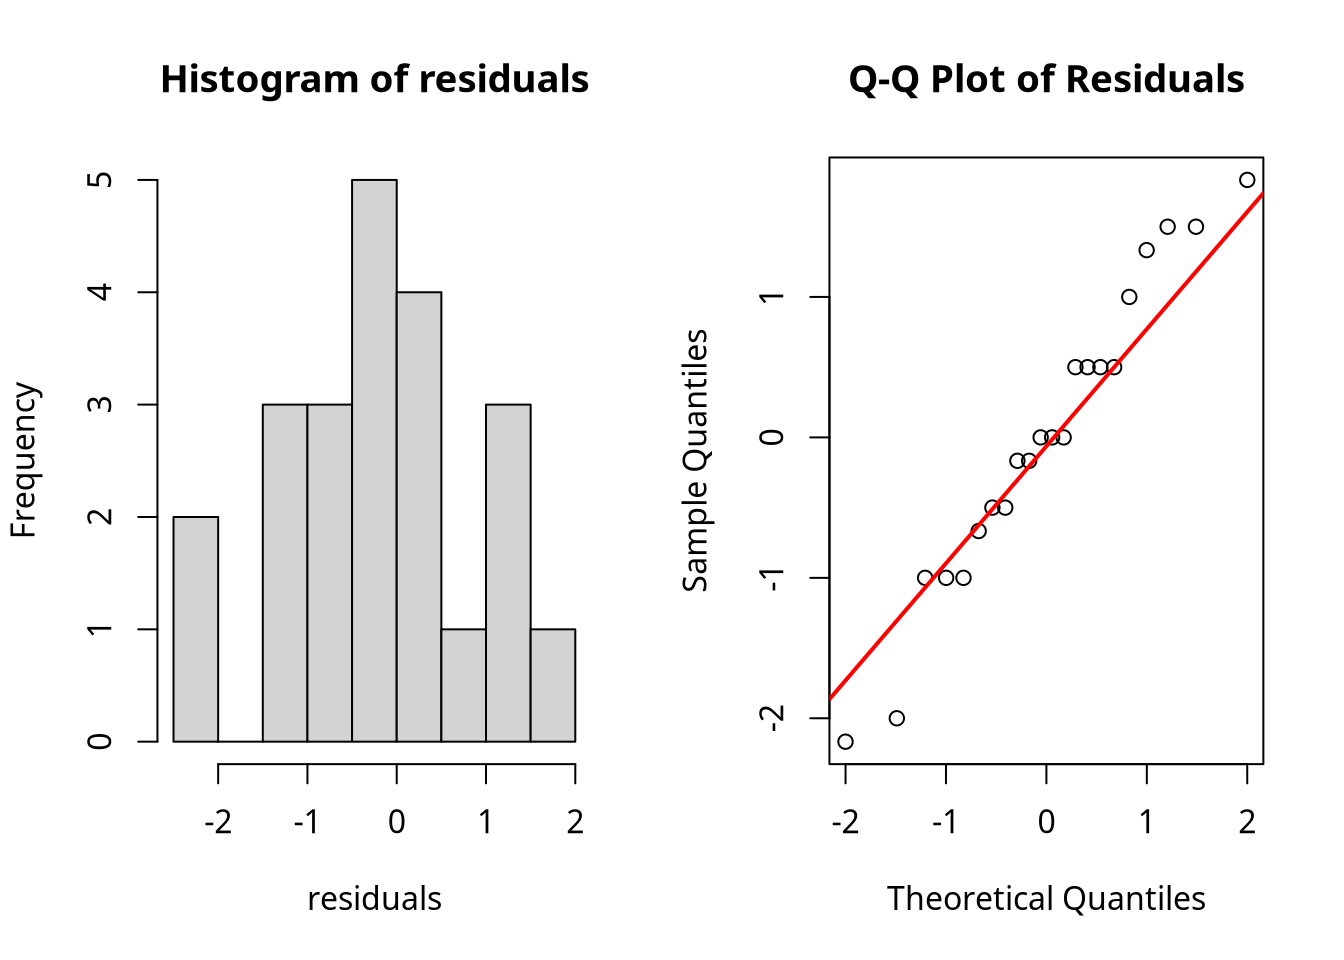
\includegraphics[keepaspectratio]{01-contrastes-parametricos-practicas_files/figure-pdf/unnamed-chunk-33-1.pdf}}

\begin{Shaded}
\begin{Highlighting}[]
\FunctionTok{tidy}\NormalTok{(}\FunctionTok{shapiro.test}\NormalTok{(residuals)) }\SpecialCharTok{|\textgreater{}} 
\FunctionTok{kable}\NormalTok{()}
\end{Highlighting}
\end{Shaded}

  \begin{longtable}[]{@{}rrl@{}}
  \toprule\noalign{}
  statistic & p.value & method \\
  \midrule\noalign{}
  \endhead
  \bottomrule\noalign{}
  \endlastfoot
  0.967452 & 0.6521599 & Shapiro-Wilk normality test \\
  \end{longtable}

  Tanto el histograma como el gráfico de cuantiles no muestran una
  desviación significativa de una distribución normal, y como el p-valor
  del contraste de normalidad es mayor que el nivel de significación
  \(0.05\), se asume que los residuos siguen una distribución normal.
\item
  Homogeneidad de varianzas. Aplicamos el test de Levene para la
  comparación de varianzas.

\begin{Shaded}
\begin{Highlighting}[]
\FunctionTok{library}\NormalTok{(car)}
\FunctionTok{tidy}\NormalTok{(}\FunctionTok{leveneTest}\NormalTok{(Perdida\_peso }\SpecialCharTok{\textasciitilde{}}\NormalTok{ Dieta }\SpecialCharTok{*}\NormalTok{ Farmaco, }\AttributeTok{data =}\NormalTok{ df)) }\SpecialCharTok{|\textgreater{}} 
\FunctionTok{kable}\NormalTok{()}
\end{Highlighting}
\end{Shaded}

  \begin{longtable}[]{@{}rrrr@{}}
  \toprule\noalign{}
  statistic & p.value & df & df.residual \\
  \midrule\noalign{}
  \endhead
  \bottomrule\noalign{}
  \endlastfoot
  0.2715568 & 0.845079 & 3 & 18 \\
  \end{longtable}

  Como el p-valor es mayor que el nivel de significación \(0.05\) se
  acepta la hipótesis nula y se asume homogeneidad de varianzas.

  Así pues, se cumplen los requisitos para el contraste de ANOVA.
\end{enumerate}

Finalmente hacemos una comparación de medias por pares para ver entre
qué grupos hay diferencias estadísticamente significativas.

\begin{Shaded}
\begin{Highlighting}[]
\FunctionTok{tidy}\NormalTok{(}\FunctionTok{TukeyHSD}\NormalTok{(anova)) }\SpecialCharTok{|\textgreater{}} 
    \FunctionTok{kable}\NormalTok{()}
\end{Highlighting}
\end{Shaded}

\begin{longtable}[]{@{}
  >{\raggedright\arraybackslash}p{(\linewidth - 12\tabcolsep) * \real{0.1750}}
  >{\raggedright\arraybackslash}p{(\linewidth - 12\tabcolsep) * \real{0.1500}}
  >{\raggedleft\arraybackslash}p{(\linewidth - 12\tabcolsep) * \real{0.1375}}
  >{\raggedleft\arraybackslash}p{(\linewidth - 12\tabcolsep) * \real{0.1250}}
  >{\raggedleft\arraybackslash}p{(\linewidth - 12\tabcolsep) * \real{0.1375}}
  >{\raggedleft\arraybackslash}p{(\linewidth - 12\tabcolsep) * \real{0.1250}}
  >{\raggedleft\arraybackslash}p{(\linewidth - 12\tabcolsep) * \real{0.1500}}@{}}
\toprule\noalign{}
\begin{minipage}[b]{\linewidth}\raggedright
term
\end{minipage} & \begin{minipage}[b]{\linewidth}\raggedright
contrast
\end{minipage} & \begin{minipage}[b]{\linewidth}\raggedleft
null.value
\end{minipage} & \begin{minipage}[b]{\linewidth}\raggedleft
estimate
\end{minipage} & \begin{minipage}[b]{\linewidth}\raggedleft
conf.low
\end{minipage} & \begin{minipage}[b]{\linewidth}\raggedleft
conf.high
\end{minipage} & \begin{minipage}[b]{\linewidth}\raggedleft
adj.p.value
\end{minipage} \\
\midrule\noalign{}
\endhead
\bottomrule\noalign{}
\endlastfoot
Dieta & Si-No & 0 & 5.090909 & 4.0493279 & 6.132490 & 0.0000000 \\
Farmaco & Si-No & 0 & 7.083333 & 6.0374212 & 8.129245 & 0.0000000 \\
Dieta:Farmaco & Si:No-No:No & 0 & 3.000000 & 0.9216855 & 5.078315 &
0.0035774 \\
Dieta:Farmaco & No:Si-No:No & 0 & 5.166667 & 3.1768320 & 7.156501 &
0.0000046 \\
Dieta:Farmaco & Si:Si-No:No & 0 & 12.000000 & 10.0101653 & 13.989835 &
0.0000000 \\
Dieta:Farmaco & No:Si-Si:No & 0 & 2.166667 & 0.1768320 & 4.156501 &
0.0300974 \\
Dieta:Farmaco & Si:Si-Si:No & 0 & 9.000000 & 7.0101653 & 10.989835 &
0.0000000 \\
Dieta:Farmaco & Si:Si-No:Si & 0 & 6.833333 & 4.9361004 & 8.730566 &
0.0000000 \\
\end{longtable}

Se observan diferencias estadísticamente significativas entre todos los
grupos de comparación.

\begin{Shaded}
\begin{Highlighting}[]
\FunctionTok{tidy}\NormalTok{(}\FunctionTok{TukeyHSD}\NormalTok{(anova)) }\SpecialCharTok{|\textgreater{}} 
    \FunctionTok{ggplot}\NormalTok{(}\FunctionTok{aes}\NormalTok{(}\AttributeTok{x =}\NormalTok{ contrast, }\AttributeTok{y =}\NormalTok{ estimate)) }\SpecialCharTok{+}
    \FunctionTok{geom\_errorbar}\NormalTok{(}\FunctionTok{aes}\NormalTok{(}\AttributeTok{ymin =}\NormalTok{ conf.low, }\AttributeTok{ymax =}\NormalTok{ conf.high), }\AttributeTok{width =} \FloatTok{0.2}\NormalTok{, }\AttributeTok{color =} \StringTok{"blue"}\NormalTok{) }\SpecialCharTok{+}
    \FunctionTok{geom\_point}\NormalTok{(}\AttributeTok{size =} \DecValTok{3}\NormalTok{, }\AttributeTok{color =} \StringTok{"red"}\NormalTok{) }\SpecialCharTok{+}
    \FunctionTok{geom\_hline}\NormalTok{(}\AttributeTok{yintercept =} \DecValTok{0}\NormalTok{, }\AttributeTok{linetype =} \StringTok{"dashed"}\NormalTok{)}
\end{Highlighting}
\end{Shaded}

\pandocbounded{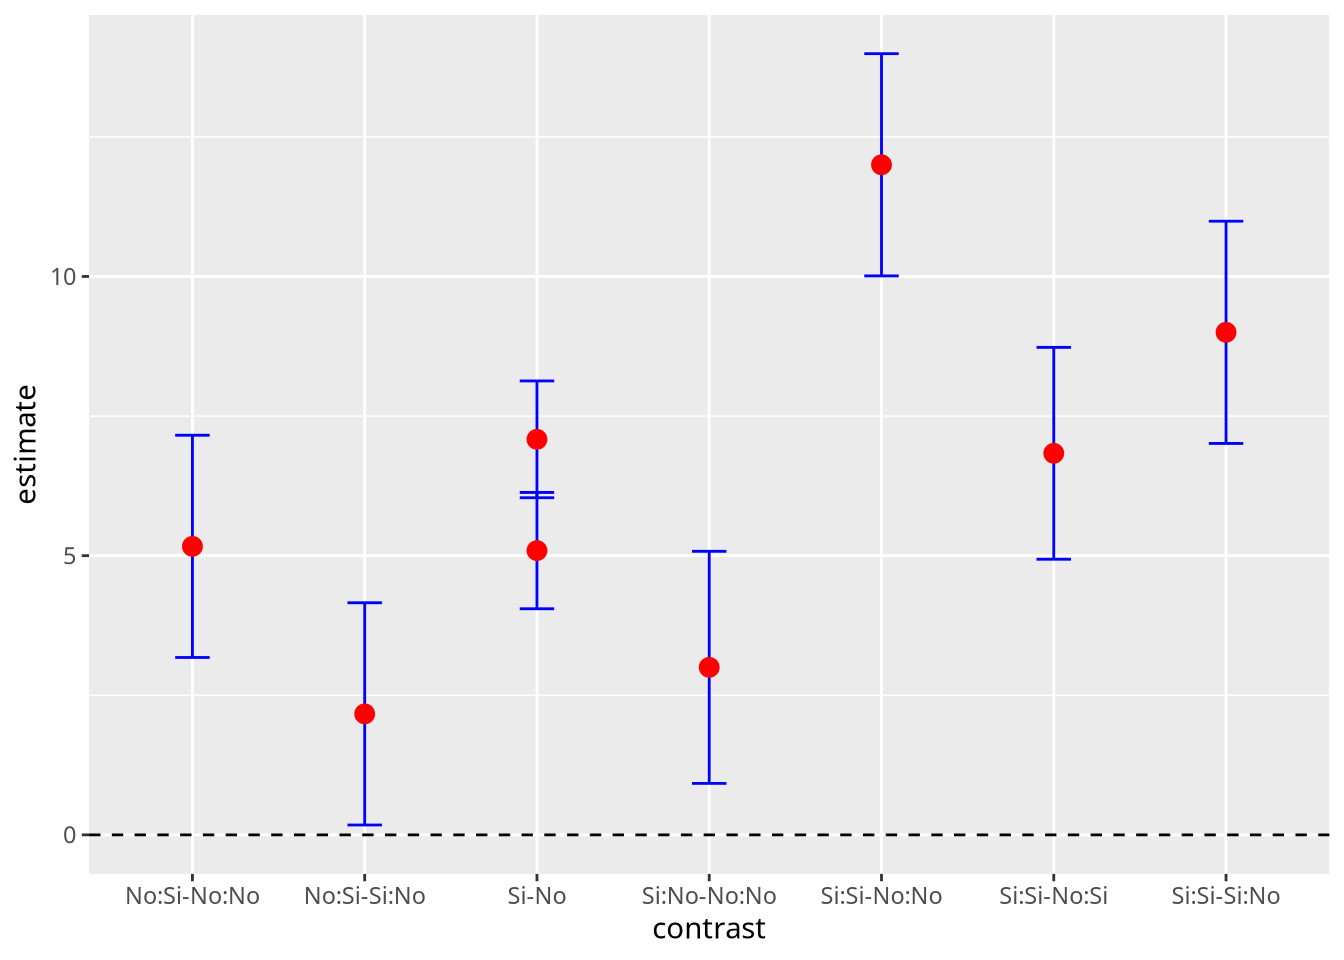
\includegraphics[keepaspectratio]{01-contrastes-parametricos-practicas_files/figure-pdf/unnamed-chunk-36-1.pdf}}

\end{tcolorbox}

\begin{exercise}[]\protect\hypertarget{exr-regresion-metabolismo-alcohol}{}\label{exr-regresion-metabolismo-alcohol}

Después de tomar un litro de vino se ha medido la concentración de
alcohol en la sangre en distintos instantes, obteniendo los siguientes
datos

\[
\begin{array}{lrrrrrrr}
\hline 
\mbox{Tiempo después (minutos)} & 30 & 60 & 90 & 120 & 150 & 180 & 210\\ 
\mbox{Alcohol (gramos/litro)} & 1.6 & 1.7 & 1.5 & 1.1 & 0.7 & 0.2 & 2.1\\
\hline
\end{array}
\]

\begin{enumerate}
\def\labelenumi{\alph{enumi}.}
\item
  Crear un data frame con los datos del tiempo y la concentración de
  alcohol.

  \begin{tcolorbox}[enhanced jigsaw, breakable, opacityback=0, colbacktitle=quarto-callout-tip-color!10!white, colframe=quarto-callout-tip-color-frame, left=2mm, titlerule=0mm, coltitle=black, colback=white, bottomtitle=1mm, toptitle=1mm, opacitybacktitle=0.6, title=\textcolor{quarto-callout-tip-color}{\faLightbulb}\hspace{0.5em}{Solución}, leftrule=.75mm, bottomrule=.15mm, toprule=.15mm, rightrule=.15mm, arc=.35mm]

\begin{Shaded}
\begin{Highlighting}[]
\NormalTok{df }\OtherTok{\textless{}{-}} \FunctionTok{data.frame}\NormalTok{(}
    \AttributeTok{Tiempo =} \FunctionTok{c}\NormalTok{(}\DecValTok{30}\NormalTok{, }\DecValTok{60}\NormalTok{, }\DecValTok{90}\NormalTok{, }\DecValTok{120}\NormalTok{, }\DecValTok{150}\NormalTok{, }\DecValTok{180}\NormalTok{, }\DecValTok{210}\NormalTok{),}
    \AttributeTok{Alcohol =} \FunctionTok{c}\NormalTok{(}\FloatTok{1.6}\NormalTok{, }\FloatTok{1.7}\NormalTok{, }\FloatTok{1.5}\NormalTok{, }\FloatTok{1.1}\NormalTok{, }\FloatTok{0.7}\NormalTok{, }\FloatTok{0.2}\NormalTok{, }\FloatTok{2.1}\NormalTok{)}
\NormalTok{)}
\NormalTok{df}
\end{Highlighting}
\end{Shaded}

\begin{verbatim}
  Tiempo Alcohol
1     30     1.6
2     60     1.7
3     90     1.5
4    120     1.1
5    150     0.7
6    180     0.2
7    210     2.1
\end{verbatim}

  \end{tcolorbox}
\item
  Calcular el coeficiente de correlación lineal. ¿Existe relación lineal
  entre la concentración de alcohol y el tiempo que pasa?

  \begin{tcolorbox}[enhanced jigsaw, breakable, opacityback=0, colbacktitle=quarto-callout-tip-color!10!white, colframe=quarto-callout-tip-color-frame, left=2mm, titlerule=0mm, coltitle=black, colback=white, bottomtitle=1mm, toptitle=1mm, opacitybacktitle=0.6, title=\textcolor{quarto-callout-tip-color}{\faLightbulb}\hspace{0.5em}{Solución}, leftrule=.75mm, bottomrule=.15mm, toprule=.15mm, rightrule=.15mm, arc=.35mm]

  Para calcular el coeficiente de correlación lineal de Pearson se puede
  utilar la función
  \href{https://www.rdocumentation.org/packages/stats/versions/3.6.2/topics/cor}{\texttt{cor}}
  del paquete \texttt{stats}.

\begin{Shaded}
\begin{Highlighting}[]
\FunctionTok{cor}\NormalTok{(df}\SpecialCharTok{$}\NormalTok{Tiempo, df}\SpecialCharTok{$}\NormalTok{Alcohol)}
\end{Highlighting}
\end{Shaded}

\begin{verbatim}
[1] -0.2730367
\end{verbatim}

  El valore del coeficiente de correlación lineal es muy bajo, por lo
  que aparentemente no hay relación lineal entre la concentración de
  alcohol en sangre y el tiempo que pasa.

  \end{tcolorbox}
\item
  Dibujar el diagrama de dispersión correspondiente y la recta de
  regresión de la concentración de alcohol sobre el tiempo. ¿Por qué el
  ajuste es tan malo?

  \begin{tcolorbox}[enhanced jigsaw, breakable, opacityback=0, colbacktitle=quarto-callout-tip-color!10!white, colframe=quarto-callout-tip-color-frame, left=2mm, titlerule=0mm, coltitle=black, colback=white, bottomtitle=1mm, toptitle=1mm, opacitybacktitle=0.6, title=\textcolor{quarto-callout-tip-color}{\faLightbulb}\hspace{0.5em}{Solución}, leftrule=.75mm, bottomrule=.15mm, toprule=.15mm, rightrule=.15mm, arc=.35mm]

\begin{Shaded}
\begin{Highlighting}[]
\FunctionTok{library}\NormalTok{(ggplot2)}
\FunctionTok{ggplot}\NormalTok{(df, }\FunctionTok{aes}\NormalTok{(}\AttributeTok{x =}\NormalTok{ Tiempo, }\AttributeTok{y =}\NormalTok{ Alcohol)) }\SpecialCharTok{+}
    \FunctionTok{geom\_point}\NormalTok{(}\AttributeTok{col =} \StringTok{"red"}\NormalTok{) }\SpecialCharTok{+}
    \FunctionTok{geom\_smooth}\NormalTok{(}\AttributeTok{method =} \StringTok{"lm"}\NormalTok{) }\SpecialCharTok{+}
    \FunctionTok{labs}\NormalTok{(}\AttributeTok{title =} \StringTok{"Diagrama de dispersión"}\NormalTok{, }\AttributeTok{x =} \StringTok{"Tiempo en minutos"}\NormalTok{, }\AttributeTok{y =} \StringTok{"Concentración de alcohol en sangre (g/l)"}\NormalTok{)}
\end{Highlighting}
\end{Shaded}

\begin{verbatim}
`geom_smooth()` using formula = 'y ~ x'
\end{verbatim}

  \pandocbounded{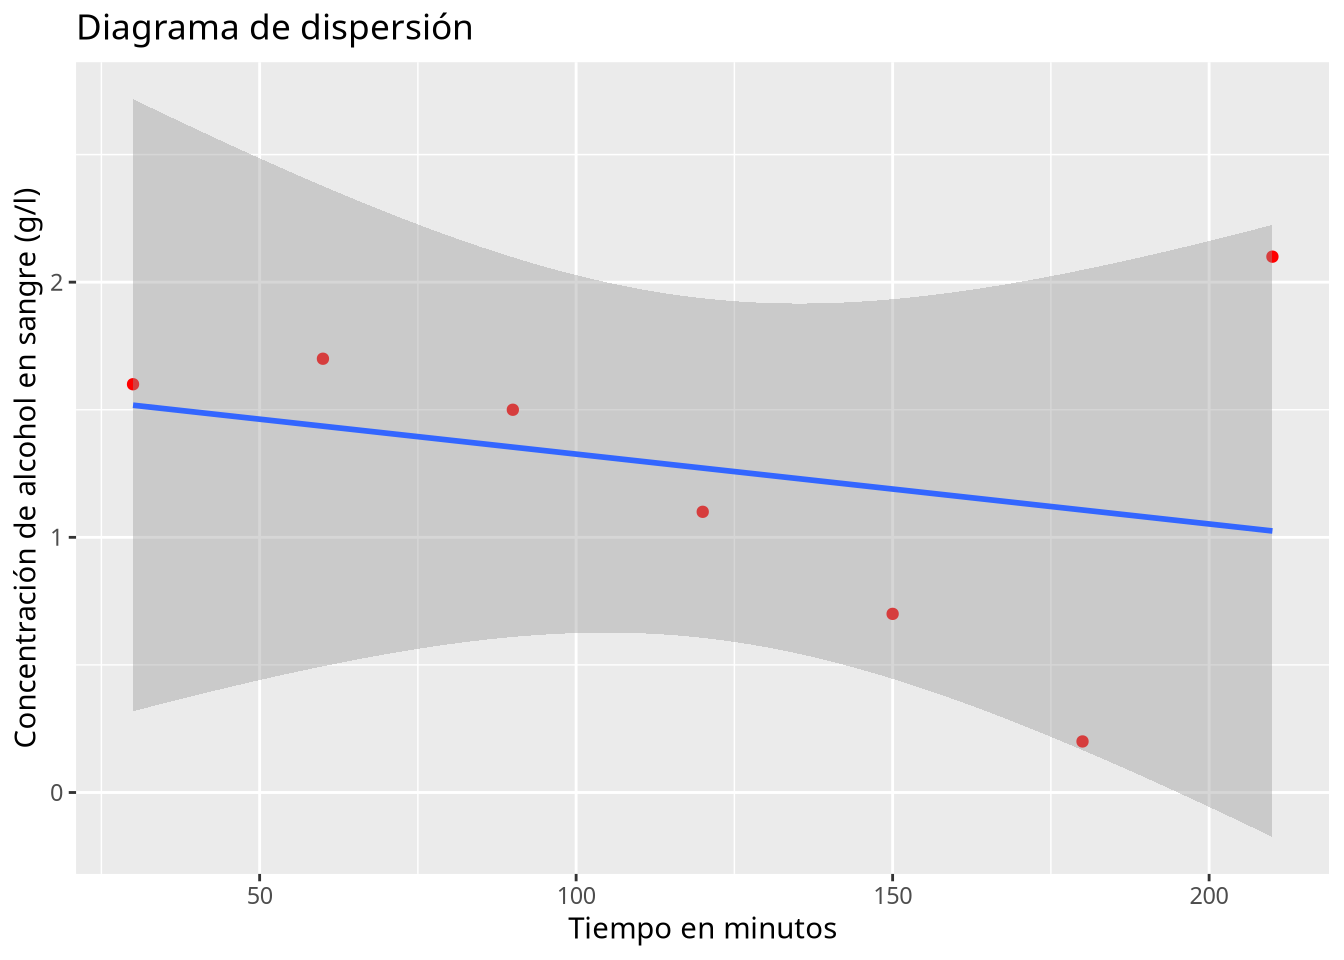
\includegraphics[keepaspectratio]{01-contrastes-parametricos-practicas_files/figure-pdf/unnamed-chunk-39-1.pdf}}

  El ajuste es malo porque hay un dato atípico que no sigue la misma
  tendencia que el resto.

  \end{tcolorbox}
\item
  Eliminar el dato atípico y calcular la recta de la concentración de
  alcohol sobre el tiempo. ¿Ha mejorado el modelo?

  \begin{tcolorbox}[enhanced jigsaw, breakable, opacityback=0, colbacktitle=quarto-callout-tip-color!10!white, colframe=quarto-callout-tip-color-frame, left=2mm, titlerule=0mm, coltitle=black, colback=white, bottomtitle=1mm, toptitle=1mm, opacitybacktitle=0.6, title=\textcolor{quarto-callout-tip-color}{\faLightbulb}\hspace{0.5em}{Solución}, leftrule=.75mm, bottomrule=.15mm, toprule=.15mm, rightrule=.15mm, arc=.35mm]

\begin{Shaded}
\begin{Highlighting}[]
\CommentTok{\# Eliminamos el dato atípico que está en la fila }
\NormalTok{df }\OtherTok{\textless{}{-}}\NormalTok{ df[}\SpecialCharTok{{-}}\FunctionTok{c}\NormalTok{(}\DecValTok{7}\NormalTok{), ]}
\NormalTok{recta\_alcohol\_tiempo }\OtherTok{\textless{}{-}} \FunctionTok{lm}\NormalTok{(Alcohol }\SpecialCharTok{\textasciitilde{}}\NormalTok{ Tiempo, df) }
\FunctionTok{summary}\NormalTok{(recta\_alcohol\_tiempo)}
\end{Highlighting}
\end{Shaded}

\begin{verbatim}

Call:
lm(formula = Alcohol ~ Tiempo, data = df)

Residuals:
       1        2        3        4        5        6 
-0.27619  0.12095  0.21810  0.11524  0.01238 -0.19048 

Coefficients:
             Estimate Std. Error t value Pr(>|t|)    
(Intercept)  2.173333   0.201927  10.763 0.000423 ***
Tiempo      -0.009905   0.001728  -5.731 0.004591 ** 
---
Signif. codes:  0 '***' 0.001 '**' 0.01 '*' 0.05 '.' 0.1 ' ' 1

Residual standard error: 0.2169 on 4 degrees of freedom
Multiple R-squared:  0.8914,    Adjusted R-squared:  0.8643 
F-statistic: 32.84 on 1 and 4 DF,  p-value: 0.004591
\end{verbatim}

  La recta de regresión de la concentración de alcohol en sangre sobre
  el tiempo es
  \(\textsf{alcohol}= 2.1733333 + -0.0099048 \textsf{tiempo}\).

  El modelo ha mejorado notablemente ya que ahora el coeficiente de
  determinación lineal \(R^2=0.8914286\), que está muy próximo a 1.

  \end{tcolorbox}
\item
  Según el modelo de regresión lineal, ¿a qué velocidad metaboliza esta
  persona el alcohol?

  \begin{tcolorbox}[enhanced jigsaw, breakable, opacityback=0, colbacktitle=quarto-callout-tip-color!10!white, colframe=quarto-callout-tip-color-frame, left=2mm, titlerule=0mm, coltitle=black, colback=white, bottomtitle=1mm, toptitle=1mm, opacitybacktitle=0.6, title=\textcolor{quarto-callout-tip-color}{\faLightbulb}\hspace{0.5em}{Solución}, leftrule=.75mm, bottomrule=.15mm, toprule=.15mm, rightrule=.15mm, arc=.35mm]

\begin{Shaded}
\begin{Highlighting}[]
\FunctionTok{cat}\NormalTok{(}\FunctionTok{paste}\NormalTok{(}\StringTok{"Coeficiente de regresión de la concentración de alchol sobre el tiempo:"}\NormalTok{, recta\_alcohol\_tiempo}\SpecialCharTok{$}\NormalTok{coefficients[[}\StringTok{"Tiempo"}\NormalTok{]]))}
\end{Highlighting}
\end{Shaded}

\begin{verbatim}
Coeficiente de regresión de la concentración de alchol sobre el tiempo: -0.00990476190476191
\end{verbatim}

  Así pues, la velocidad de metabolización del alcohol es 0.0099048
  g/l\(\cdot\)min.

  \end{tcolorbox}
\item
  Si la concentración máxima de alcohol en la sangre que permite la ley
  para poder conducir es \(0.3\) g/l, ¿cuánto tiempo habrá que esperar
  después de tomarse un litro de vino para poder conducir sin infringir
  la ley? ¿Es fiable esta predicción?

  \begin{tcolorbox}[enhanced jigsaw, breakable, opacityback=0, colbacktitle=quarto-callout-tip-color!10!white, colframe=quarto-callout-tip-color-frame, left=2mm, titlerule=0mm, coltitle=black, colback=white, bottomtitle=1mm, toptitle=1mm, opacitybacktitle=0.6, title=\textcolor{quarto-callout-tip-color}{\faLightbulb}\hspace{0.5em}{Solución}, leftrule=.75mm, bottomrule=.15mm, toprule=.15mm, rightrule=.15mm, arc=.35mm]

  Como ahora queremos predecir el tiempo, necesitamos calcular la recta
  de regresión del tiempo sobre la concentración de alcohol.

\begin{Shaded}
\begin{Highlighting}[]
\NormalTok{recta\_tiempo\_alcohol }\OtherTok{\textless{}{-}} \FunctionTok{lm}\NormalTok{(Tiempo }\SpecialCharTok{\textasciitilde{}}\NormalTok{ Alcohol, df) }
\FunctionTok{predict.lm}\NormalTok{(recta\_tiempo\_alcohol, }\AttributeTok{newdata =} \FunctionTok{list}\NormalTok{(}\AttributeTok{Alcohol =} \FloatTok{0.3}\NormalTok{))}
\end{Highlighting}
\end{Shaded}

\begin{verbatim}
  1 
180 
\end{verbatim}

  Aunque el coeficiente de determinación lineal está próximo a 1, el
  tamaño muestral es demasiado pequeño para que la predicción sea
  fiable.

  \end{tcolorbox}
\end{enumerate}

\end{exercise}

\begin{exercise}[]\protect\hypertarget{exr-regresion-dieta}{}\label{exr-regresion-dieta}

El fichero \href{datos/dieta.csv}{\texttt{dieta.csv}} contiene
información sobre el los kilos perdidos con una dieta de adelgazamiento.

\begin{enumerate}
\def\labelenumi{\alph{enumi}.}
\item
  Crear un data frame con los datos de la dieta a partir del fichero
  \href{https://aprendeconalf.es/estadistica-practicas-r/datos/dieta.csv}{\texttt{dieta.csv}}.

  \begin{tcolorbox}[enhanced jigsaw, breakable, opacityback=0, colbacktitle=quarto-callout-tip-color!10!white, colframe=quarto-callout-tip-color-frame, left=2mm, titlerule=0mm, coltitle=black, colback=white, bottomtitle=1mm, toptitle=1mm, opacitybacktitle=0.6, title=\textcolor{quarto-callout-tip-color}{\faLightbulb}\hspace{0.5em}{Solución}, leftrule=.75mm, bottomrule=.15mm, toprule=.15mm, rightrule=.15mm, arc=.35mm]

\begin{Shaded}
\begin{Highlighting}[]
\FunctionTok{library}\NormalTok{(readr)}
\NormalTok{df }\OtherTok{\textless{}{-}} \FunctionTok{read\_csv}\NormalTok{(}\StringTok{"https://aprendeconalf.es/estadistica{-}practicas{-}r/datos/dieta.csv"}\NormalTok{)}
\end{Highlighting}
\end{Shaded}

\begin{verbatim}
Rows: 40 Columns: 3
-- Column specification --------------------------------------------------------
Delimiter: ","
chr (1): ejercicio
dbl (2): dias, peso.perdido

i Use `spec()` to retrieve the full column specification for this data.
i Specify the column types or set `show_col_types = FALSE` to quiet this message.
\end{verbatim}

\begin{Shaded}
\begin{Highlighting}[]
\NormalTok{df}
\end{Highlighting}
\end{Shaded}

\begin{verbatim}
# A tibble: 40 x 3
    dias peso.perdido ejercicio
   <dbl>        <dbl> <chr>    
 1    14         2.95 no       
 2    18         5.65 no       
 3    22         6.56 no       
 4    26         3.56 no       
 5    30         6.17 no       
 6    34         9.4  no       
 7    38        12.4  no       
 8    42        12.9  no       
 9    46        13.9  no       
10    50        10.8  no       
# i 30 more rows
\end{verbatim}

  \end{tcolorbox}
\item
  Dibujar el diagrama de dispersión de los kilos perdidos en función del
  número de días con la dieta. ¿Qué tipo de modelo de regresión se
  ajusta mejor a la nube de puntos?

  \begin{tcolorbox}[enhanced jigsaw, breakable, opacityback=0, colbacktitle=quarto-callout-tip-color!10!white, colframe=quarto-callout-tip-color-frame, left=2mm, titlerule=0mm, coltitle=black, colback=white, bottomtitle=1mm, toptitle=1mm, opacitybacktitle=0.6, title=\textcolor{quarto-callout-tip-color}{\faLightbulb}\hspace{0.5em}{Solución}, leftrule=.75mm, bottomrule=.15mm, toprule=.15mm, rightrule=.15mm, arc=.35mm]

\begin{Shaded}
\begin{Highlighting}[]
\FunctionTok{library}\NormalTok{(ggplot2)}
\FunctionTok{ggplot}\NormalTok{(df, }\FunctionTok{aes}\NormalTok{(}\AttributeTok{x =}\NormalTok{ dias, }\AttributeTok{y =}\NormalTok{ peso.perdido)) }\SpecialCharTok{+}
    \FunctionTok{geom\_point}\NormalTok{(}\AttributeTok{col =} \StringTok{"red"}\NormalTok{) }\SpecialCharTok{+}
    \FunctionTok{labs}\NormalTok{(}\AttributeTok{title =} \StringTok{"Diagrama de dispersión del peso perdido y los días de dieta"}\NormalTok{, }\AttributeTok{x =} \StringTok{"Días de dieta"}\NormalTok{, }\AttributeTok{y =} \StringTok{"Peso perdido en Kg"}\NormalTok{)}
\end{Highlighting}
\end{Shaded}

  \pandocbounded{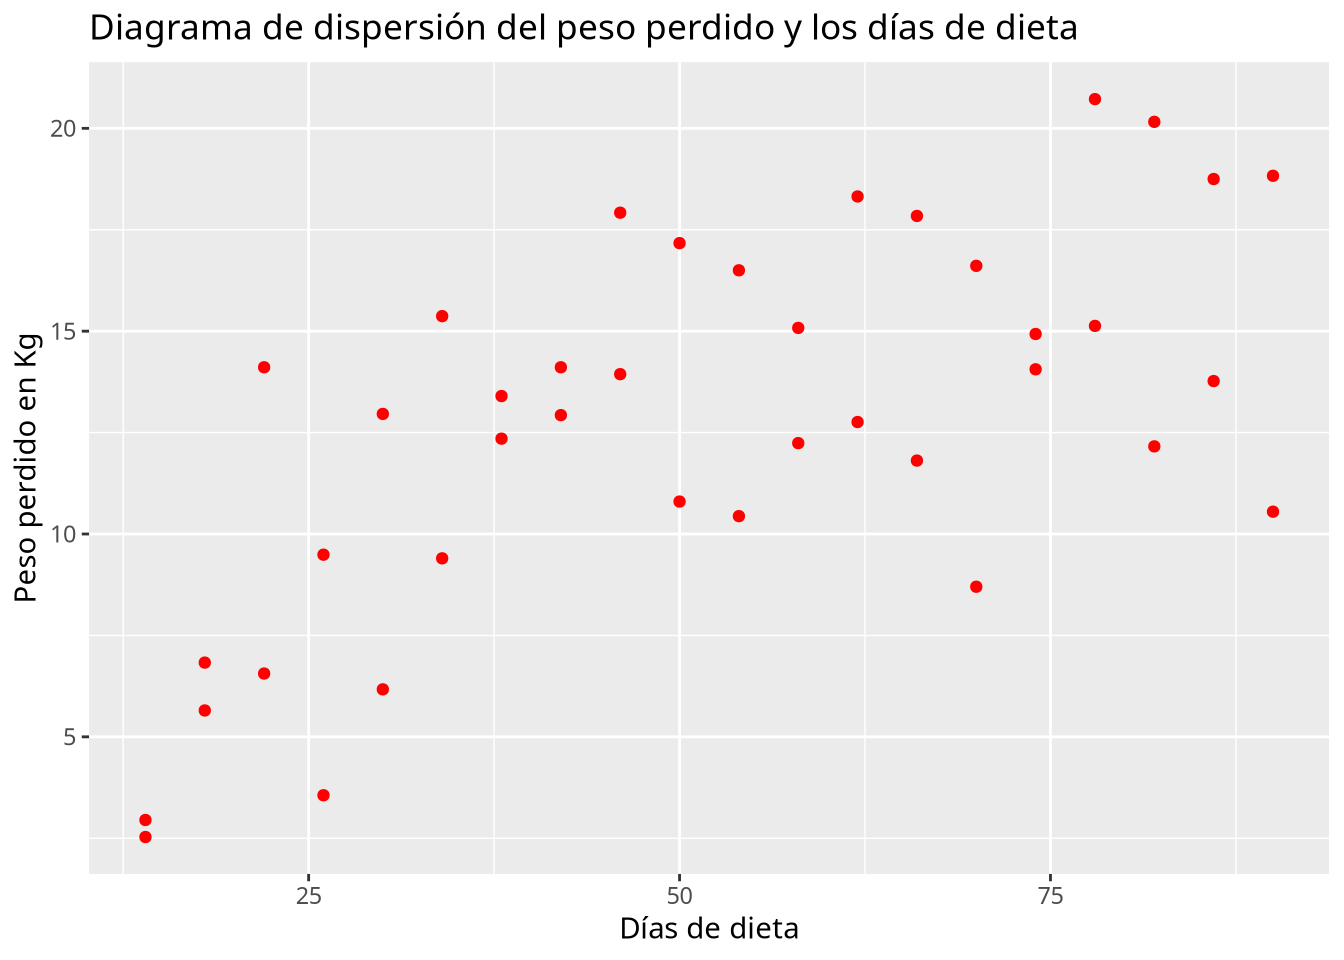
\includegraphics[keepaspectratio]{01-contrastes-parametricos-practicas_files/figure-pdf/unnamed-chunk-44-1.pdf}}

  La nube de puntos es bastante difusa aunque parece apreciarse una
  tendencia logarítmica o sigmoidal.

  \end{tcolorbox}
\item
  Calcular los coeficientes de determinación lineal, cuadrático,
  exponencial, logarítmico, potencial, inverso y sigmoidal. ¿Qué tipo de
  modelo explica mejor la relación entre los kilos perdidos y el número
  de días de dieta? ¿Qué porcentaje de la variabilidad de peso perdido
  explica el mejor modelo de regresión?

  \begin{tcolorbox}[enhanced jigsaw, breakable, opacityback=0, colbacktitle=quarto-callout-tip-color!10!white, colframe=quarto-callout-tip-color-frame, left=2mm, titlerule=0mm, coltitle=black, colback=white, bottomtitle=1mm, toptitle=1mm, opacitybacktitle=0.6, title=\textcolor{quarto-callout-tip-color}{\faLightbulb}\hspace{0.5em}{Solución}, leftrule=.75mm, bottomrule=.15mm, toprule=.15mm, rightrule=.15mm, arc=.35mm]

\begin{Shaded}
\begin{Highlighting}[]
\FunctionTok{library}\NormalTok{(dplyr)}
\FunctionTok{library}\NormalTok{(tidyr)}
\FunctionTok{library}\NormalTok{(purrr)}
\FunctionTok{library}\NormalTok{(broom)}
\FunctionTok{library}\NormalTok{(kableExtra)}
\end{Highlighting}
\end{Shaded}

\begin{verbatim}

Adjuntando el paquete: 'kableExtra'
\end{verbatim}

\begin{verbatim}
The following object is masked from 'package:dplyr':

    group_rows
\end{verbatim}

\begin{Shaded}
\begin{Highlighting}[]
\CommentTok{\# Construimos un data frame con el ajuste de los modelos.}
\NormalTok{modelos }\OtherTok{\textless{}{-}} \FunctionTok{tibble}\NormalTok{(}
        \AttributeTok{Lineal =} \FunctionTok{list}\NormalTok{(}\FunctionTok{lm}\NormalTok{(peso.perdido }\SpecialCharTok{\textasciitilde{}}\NormalTok{ dias, df)),}
        \AttributeTok{Cuadratico =} \FunctionTok{list}\NormalTok{(}\FunctionTok{lm}\NormalTok{(peso.perdido }\SpecialCharTok{\textasciitilde{}}\NormalTok{ dias }\SpecialCharTok{+} \FunctionTok{I}\NormalTok{(dias}\SpecialCharTok{\^{}}\DecValTok{2}\NormalTok{), df)),}
        \AttributeTok{Exponencial =} \FunctionTok{list}\NormalTok{(}\FunctionTok{lm}\NormalTok{(}\FunctionTok{log}\NormalTok{(peso.perdido) }\SpecialCharTok{\textasciitilde{}}\NormalTok{ dias, df)),}
        \AttributeTok{Logaritmico =} \FunctionTok{list}\NormalTok{(}\FunctionTok{lm}\NormalTok{(peso.perdido }\SpecialCharTok{\textasciitilde{}} \FunctionTok{log}\NormalTok{(dias), df)),}
        \AttributeTok{Potencial =} \FunctionTok{list}\NormalTok{(}\FunctionTok{lm}\NormalTok{(}\FunctionTok{log}\NormalTok{(peso.perdido) }\SpecialCharTok{\textasciitilde{}} \FunctionTok{log}\NormalTok{(dias), df)),}
        \AttributeTok{Inverso =} \FunctionTok{list}\NormalTok{(}\FunctionTok{lm}\NormalTok{(peso.perdido }\SpecialCharTok{\textasciitilde{}} \FunctionTok{I}\NormalTok{(}\DecValTok{1}\SpecialCharTok{/}\NormalTok{dias), df)),}
        \AttributeTok{Sigmoidal =} \FunctionTok{list}\NormalTok{(}\FunctionTok{lm}\NormalTok{(}\FunctionTok{log}\NormalTok{(peso.perdido) }\SpecialCharTok{\textasciitilde{}} \FunctionTok{I}\NormalTok{(}\DecValTok{1}\SpecialCharTok{/}\NormalTok{dias), df)),}
\NormalTok{    )  }\SpecialCharTok{|\textgreater{}} 
    \CommentTok{\# }
    \CommentTok{\# Reestructuramos el data frame para tener todos los modelos en la misma columna.}
    \FunctionTok{pivot\_longer}\NormalTok{(}\FunctionTok{everything}\NormalTok{(), }\AttributeTok{names\_to =} \StringTok{"Tipo\_Modelo"}\NormalTok{, }\AttributeTok{values\_to =} \StringTok{"Modelo"}\NormalTok{)  }\SpecialCharTok{|\textgreater{}} 
    \CommentTok{\# Obtenemos un resumen del ajuste de cada modelo en formato organizado (se obtiene una lista con los parámetros que describen el ajuste de cada modelo).}
    \FunctionTok{mutate}\NormalTok{(}\AttributeTok{Resumen =} \FunctionTok{map}\NormalTok{(Modelo, glance)) }\SpecialCharTok{|\textgreater{}} 
    \CommentTok{\# Desanidamos el resumen (se obtiene una columna para cada parámetro del resumen del ajuste de los modelos).}
    \FunctionTok{unnest}\NormalTok{(Resumen)  }\SpecialCharTok{|\textgreater{}} 
    \CommentTok{\# Ordenamos el data frame por el coeficiente de determinación.}
    \FunctionTok{arrange}\NormalTok{(}\SpecialCharTok{{-}}\NormalTok{r.squared)}

\NormalTok{modelos  }\SpecialCharTok{|\textgreater{}}
    \FunctionTok{select}\NormalTok{(Tipo\_Modelo, r.squared)  }\SpecialCharTok{|\textgreater{}} 
    \FunctionTok{kable}\NormalTok{(}\AttributeTok{col.names =} \FunctionTok{c}\NormalTok{(}\StringTok{"Tipo de Modelo"}\NormalTok{, }\StringTok{"R²"}\NormalTok{)) }\SpecialCharTok{|\textgreater{}}
    \FunctionTok{kable\_styling}\NormalTok{(}\AttributeTok{full\_width =}\NormalTok{ F)}
\end{Highlighting}
\end{Shaded}

  \begin{longtable*}[t]{lr}
  \toprule
  Tipo de Modelo & R²\\
  \midrule
  Sigmoidal & 0.6662170\\
  Potencial & 0.5684490\\
  Inverso & 0.5583853\\
  Cuadratico & 0.5397848\\
  Logaritmico & 0.5254856\\
  \addlinespace
  Lineal & 0.4356390\\
  Exponencial & 0.4308936\\
  \bottomrule
  \end{longtable*}

  El mejor modelo es el Sigmoidal que explica el 66.6216965388749\% de
  la variabilidad del peso perdido.

  \end{tcolorbox}
\item
  Dibujar el diagrama de dispersión de los kilos perdidos en función del
  número de días con la dieta según si la persona hace ejercicio o no.
  ¿Qué conclusiones se pueden sacar?

  \begin{tcolorbox}[enhanced jigsaw, breakable, opacityback=0, colbacktitle=quarto-callout-tip-color!10!white, colframe=quarto-callout-tip-color-frame, left=2mm, titlerule=0mm, coltitle=black, colback=white, bottomtitle=1mm, toptitle=1mm, opacitybacktitle=0.6, title=\textcolor{quarto-callout-tip-color}{\faLightbulb}\hspace{0.5em}{Solución}, leftrule=.75mm, bottomrule=.15mm, toprule=.15mm, rightrule=.15mm, arc=.35mm]

\begin{Shaded}
\begin{Highlighting}[]
\FunctionTok{library}\NormalTok{(ggplot2)}
\FunctionTok{ggplot}\NormalTok{(df, }\FunctionTok{aes}\NormalTok{(}\AttributeTok{x =}\NormalTok{ dias, }\AttributeTok{y =}\NormalTok{ peso.perdido, }\AttributeTok{color =}\NormalTok{ ejercicio)) }\SpecialCharTok{+}
    \FunctionTok{geom\_point}\NormalTok{() }\SpecialCharTok{+}
    \FunctionTok{labs}\NormalTok{(}\AttributeTok{title =} \StringTok{"Diagrama de dispersión del peso perdido y los días de dieta"}\NormalTok{, }\AttributeTok{x =} \StringTok{"Días de dieta"}\NormalTok{, }\AttributeTok{y =} \StringTok{"Peso perdido en Kg"}\NormalTok{)}
\end{Highlighting}
\end{Shaded}

  \pandocbounded{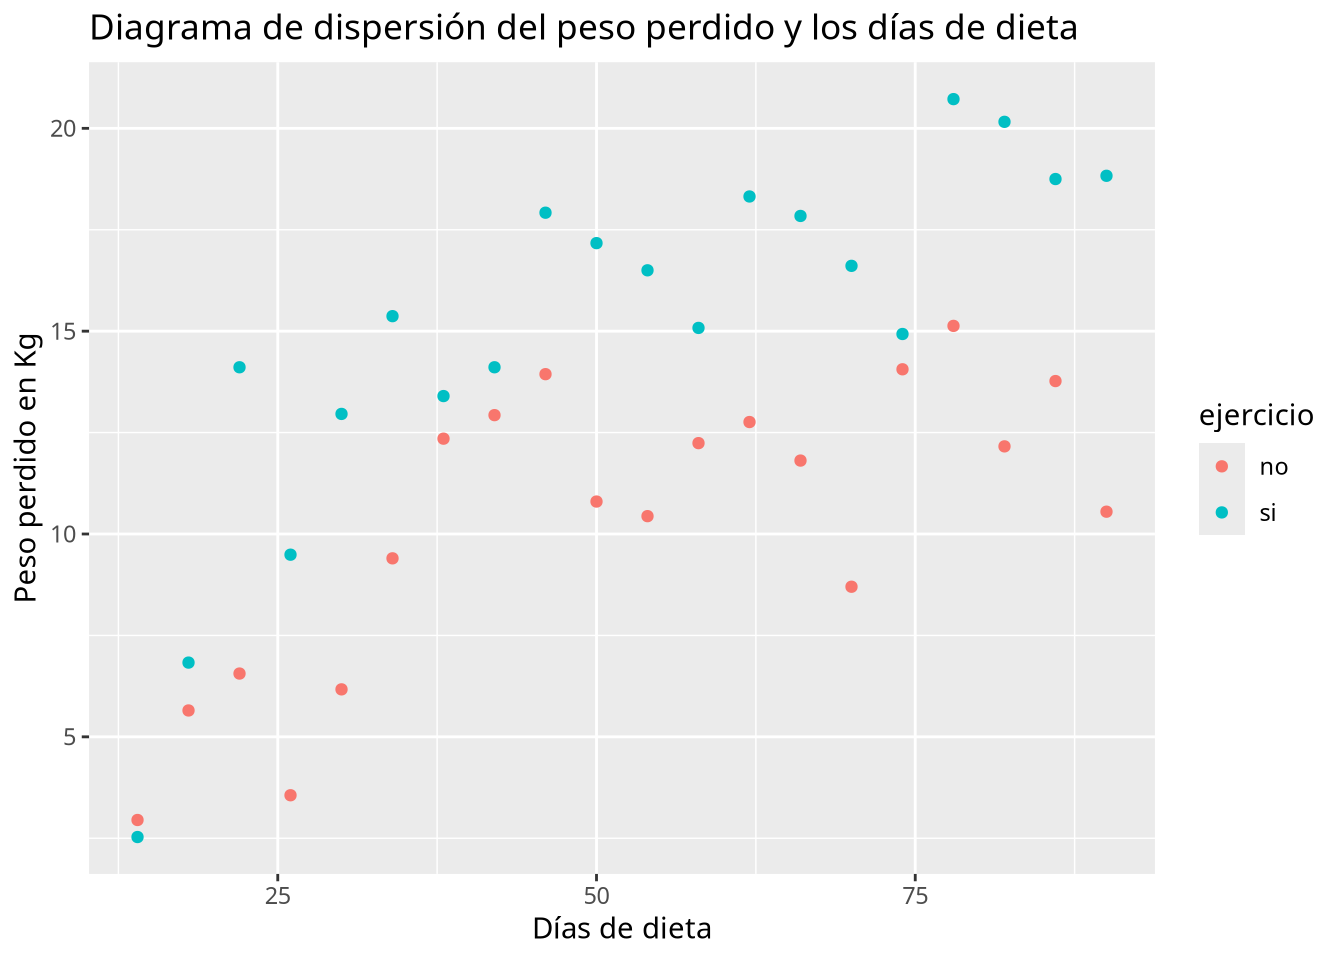
\includegraphics[keepaspectratio]{01-contrastes-parametricos-practicas_files/figure-pdf/unnamed-chunk-46-1.pdf}}

  Claramente la nube de puntos de las personas que hacen ejercicio está
  por encima de la de los que no hacen ejercicio, lo que indica que
  hacer ejercicio favorece la pérdida de peso. Los más razonable es
  construir modelos de regresión para cada grupo.

  \end{tcolorbox}
\item
  ¿Qué tipo de modelo explica mejor la relación entre el peso perdido y
  los días de dieta en el grupo de las personas que hacen ejercicio? ¿Y
  en el grupo de las que no hacen ejercicio? ¿Han mejorado los modelos
  con respecto al modelo anterior?

  \begin{tcolorbox}[enhanced jigsaw, breakable, opacityback=0, colbacktitle=quarto-callout-tip-color!10!white, colframe=quarto-callout-tip-color-frame, left=2mm, titlerule=0mm, coltitle=black, colback=white, bottomtitle=1mm, toptitle=1mm, opacitybacktitle=0.6, title=\textcolor{quarto-callout-tip-color}{\faLightbulb}\hspace{0.5em}{Solución}, leftrule=.75mm, bottomrule=.15mm, toprule=.15mm, rightrule=.15mm, arc=.35mm]

\begin{Shaded}
\begin{Highlighting}[]
\NormalTok{modelos }\OtherTok{\textless{}{-}}\NormalTok{ df  }\SpecialCharTok{|\textgreater{}} 
    \CommentTok{\# Anidamos por la columna ejercicio.}
    \FunctionTok{nest\_by}\NormalTok{(ejercicio)  }\SpecialCharTok{|\textgreater{}} 
    \CommentTok{\# Ajustamos los modelos de regresión.}
    \FunctionTok{mutate}\NormalTok{(}
        \AttributeTok{Lineal =} \FunctionTok{list}\NormalTok{(}\FunctionTok{lm}\NormalTok{(peso.perdido }\SpecialCharTok{\textasciitilde{}}\NormalTok{ dias, data)),}
        \AttributeTok{Cuadratico =} \FunctionTok{list}\NormalTok{(}\FunctionTok{lm}\NormalTok{(peso.perdido }\SpecialCharTok{\textasciitilde{}}\NormalTok{ dias }\SpecialCharTok{+} \FunctionTok{I}\NormalTok{(dias}\SpecialCharTok{\^{}}\DecValTok{2}\NormalTok{), data)),}
        \AttributeTok{Exponencial =} \FunctionTok{list}\NormalTok{(}\FunctionTok{lm}\NormalTok{(}\FunctionTok{log}\NormalTok{(peso.perdido) }\SpecialCharTok{\textasciitilde{}}\NormalTok{ dias, data)),}
        \AttributeTok{Logaritmico =} \FunctionTok{list}\NormalTok{(}\FunctionTok{lm}\NormalTok{(peso.perdido }\SpecialCharTok{\textasciitilde{}} \FunctionTok{log}\NormalTok{(dias), data)),}
        \AttributeTok{Potencial =} \FunctionTok{list}\NormalTok{(}\FunctionTok{lm}\NormalTok{(}\FunctionTok{log}\NormalTok{(peso.perdido) }\SpecialCharTok{\textasciitilde{}} \FunctionTok{log}\NormalTok{(dias), data)),}
        \AttributeTok{Inverso =} \FunctionTok{list}\NormalTok{(}\FunctionTok{lm}\NormalTok{(peso.perdido }\SpecialCharTok{\textasciitilde{}} \FunctionTok{I}\NormalTok{(}\DecValTok{1}\SpecialCharTok{/}\NormalTok{dias), data)),}
        \AttributeTok{Sigmoidal =} \FunctionTok{list}\NormalTok{(}\FunctionTok{lm}\NormalTok{(}\FunctionTok{log}\NormalTok{(peso.perdido) }\SpecialCharTok{\textasciitilde{}} \FunctionTok{I}\NormalTok{(}\DecValTok{1}\SpecialCharTok{/}\NormalTok{dias), data)),}
\NormalTok{    )  }\SpecialCharTok{|\textgreater{}} 
    \CommentTok{\# Reestructuramos el data frame para tener todos los modelos en la misma columna.}
    \FunctionTok{pivot\_longer}\NormalTok{(}\SpecialCharTok{{-}}\FunctionTok{c}\NormalTok{(ejercicio, data), }\AttributeTok{names\_to =} \StringTok{"Tipo\_Modelo"}\NormalTok{, }\AttributeTok{values\_to =} \StringTok{"Modelo"}\NormalTok{)  }\SpecialCharTok{|\textgreater{}} 
    \CommentTok{\# Obtenemos un resumen del ajuste de cada modelo en formato organizado (se obtiene una lista con los parámetros que describen el ajuste de cada modelo).}
    \FunctionTok{mutate}\NormalTok{(}\AttributeTok{Resumen =} \FunctionTok{map}\NormalTok{(Modelo, glance)) }\SpecialCharTok{|\textgreater{}} 
    \CommentTok{\# Desanidamos el resumen (se obtiene una columna para cada parámetro del resumen del ajuste de los modelos).}
    \FunctionTok{unnest}\NormalTok{(Resumen)  }\SpecialCharTok{|\textgreater{}} 
    \CommentTok{\# Ordenamos el data frame por la columna ejercicio y por el coeficiente de determinación.}
    \FunctionTok{arrange}\NormalTok{(ejercicio, }\SpecialCharTok{{-}}\NormalTok{r.squared)  }
\NormalTok{modelos }\SpecialCharTok{|\textgreater{}} 
    \FunctionTok{select}\NormalTok{(ejercicio, Tipo\_Modelo, r.squared)  }\SpecialCharTok{|\textgreater{}} 
    \FunctionTok{kable}\NormalTok{(}\AttributeTok{col.names =} \FunctionTok{c}\NormalTok{(}\StringTok{"Ejercicio"}\NormalTok{, }\StringTok{"Tipo de Modelo"}\NormalTok{, }\StringTok{"R²"}\NormalTok{)) }\SpecialCharTok{|\textgreater{}}
    \FunctionTok{pack\_rows}\NormalTok{(}\AttributeTok{index =} \FunctionTok{table}\NormalTok{(modelos}\SpecialCharTok{$}\NormalTok{ejercicio))  }\SpecialCharTok{|\textgreater{}} 
    \FunctionTok{kable\_styling}\NormalTok{(}\AttributeTok{full\_width =}\NormalTok{ F)}
\end{Highlighting}
\end{Shaded}

  \begin{longtable*}[t]{llr}
  \toprule
  Ejercicio & Tipo de Modelo & R²\\
  \midrule
  \addlinespace[0.3em]
  \multicolumn{3}{l}{\textbf{no}}\\
  \hspace{1em}no & Sigmoidal & 0.7401212\\
  \hspace{1em}no & Cuadratico & 0.7100610\\
  \hspace{1em}no & Inverso & 0.6796880\\
  \hspace{1em}no & Potencial & 0.6700051\\
  \hspace{1em}no & Logaritmico & 0.6494521\\
  \hspace{1em}no & Lineal & 0.5286338\\
  \hspace{1em}no & Exponencial & 0.5222832\\
  \addlinespace[0.3em]
  \multicolumn{3}{l}{\textbf{si}}\\
  \hspace{1em}si & Inverso & 0.8470993\\
  \hspace{1em}si & Sigmoidal & 0.8305013\\
  \hspace{1em}si & Logaritmico & 0.7885173\\
  \hspace{1em}si & Cuadratico & 0.7791671\\
  \hspace{1em}si & Potencial & 0.6704843\\
  \hspace{1em}si & Lineal & 0.6623502\\
  \hspace{1em}si & Exponencial & 0.4945564\\
  \bottomrule
  \end{longtable*}

  El mejor modelo en el grupo de los que hacen ejercicio es el inverso y
  en el grupo de los que no el sigmoidal. Los modelos han mejorado
  bastante con respecto al modelo anterior, sobre todo el del grupo de
  personas que hace ejercicio.

  \end{tcolorbox}
\item
  Construir el mejor modelo de regresión del peso perdido sobre los días
  de dieta para el grupo de las personas que hacen ejercicio y para el
  grupo de las que no.

  \begin{tcolorbox}[enhanced jigsaw, breakable, opacityback=0, colbacktitle=quarto-callout-tip-color!10!white, colframe=quarto-callout-tip-color-frame, left=2mm, titlerule=0mm, coltitle=black, colback=white, bottomtitle=1mm, toptitle=1mm, opacitybacktitle=0.6, title=\textcolor{quarto-callout-tip-color}{\faLightbulb}\hspace{0.5em}{Solución}, leftrule=.75mm, bottomrule=.15mm, toprule=.15mm, rightrule=.15mm, arc=.35mm]

  Construimos el modelo inverso para el grupo de las personas que hacen
  ejercicio.

\begin{Shaded}
\begin{Highlighting}[]
\NormalTok{inverso\_ejercicio }\OtherTok{\textless{}{-}} \FunctionTok{lm}\NormalTok{(peso.perdido }\SpecialCharTok{\textasciitilde{}} \FunctionTok{I}\NormalTok{(}\DecValTok{1}\SpecialCharTok{/}\NormalTok{dias), df[df}\SpecialCharTok{$}\NormalTok{ejercicio }\SpecialCharTok{==} \StringTok{"si"}\NormalTok{, ])}
\FunctionTok{summary}\NormalTok{(inverso\_ejercicio)}
\end{Highlighting}
\end{Shaded}

\begin{verbatim}

Call:
lm(formula = peso.perdido ~ I(1/dias), data = df[df$ejercicio == 
    "si", ])

Residuals:
    Min      1Q  Median      3Q     Max 
-3.1866 -1.3268  0.0011  0.9810  4.1456 

Coefficients:
             Estimate Std. Error t value Pr(>|t|)    
(Intercept)   21.5655     0.7653  28.181 2.42e-16 ***
I(1/dias)   -255.2249    25.5579  -9.986 9.12e-09 ***
---
Signif. codes:  0 '***' 0.001 '**' 0.01 '*' 0.05 '.' 0.1 ' ' 1

Residual standard error: 1.811 on 18 degrees of freedom
Multiple R-squared:  0.8471,    Adjusted R-squared:  0.8386 
F-statistic: 99.72 on 1 and 18 DF,  p-value: 9.123e-09
\end{verbatim}

  Y ahora el modelo sigmoidal para el grupo de las personas que no hacen
  ejercicio.

\begin{Shaded}
\begin{Highlighting}[]
\NormalTok{sigmoidal\_no\_ejercicio }\OtherTok{\textless{}{-}} \FunctionTok{lm}\NormalTok{(}\FunctionTok{log}\NormalTok{(peso.perdido) }\SpecialCharTok{\textasciitilde{}} \FunctionTok{I}\NormalTok{(}\DecValTok{1}\SpecialCharTok{/}\NormalTok{dias), df[df}\SpecialCharTok{$}\NormalTok{ejercicio }\SpecialCharTok{==} \StringTok{"no"}\NormalTok{, ])}
\FunctionTok{summary}\NormalTok{(sigmoidal\_no\_ejercicio)}
\end{Highlighting}
\end{Shaded}

\begin{verbatim}

Call:
lm(formula = log(peso.perdido) ~ I(1/dias), data = df[df$ejercicio == 
    "no", ])

Residuals:
     Min       1Q   Median       3Q      Max 
-0.66026 -0.07192  0.04678  0.13142  0.29633 

Coefficients:
            Estimate Std. Error t value Pr(>|t|)    
(Intercept)   2.8694     0.1021   28.09 2.55e-16 ***
I(1/dias)   -24.4226     3.4111   -7.16 1.15e-06 ***
---
Signif. codes:  0 '***' 0.001 '**' 0.01 '*' 0.05 '.' 0.1 ' ' 1

Residual standard error: 0.2417 on 18 degrees of freedom
Multiple R-squared:  0.7401,    Adjusted R-squared:  0.7257 
F-statistic: 51.26 on 1 and 18 DF,  p-value: 1.146e-06
\end{verbatim}

  \end{tcolorbox}
\item
  Según los mejores modelos de regresión en cada caso, ¿cuántos kilos
  perderá una persona que hace ejercicio tras 100 días de dieta? ¿Y una
  que no hace ejercicio?

  \begin{tcolorbox}[enhanced jigsaw, breakable, opacityback=0, colbacktitle=quarto-callout-tip-color!10!white, colframe=quarto-callout-tip-color-frame, left=2mm, titlerule=0mm, coltitle=black, colback=white, bottomtitle=1mm, toptitle=1mm, opacitybacktitle=0.6, title=\textcolor{quarto-callout-tip-color}{\faLightbulb}\hspace{0.5em}{Solución}, leftrule=.75mm, bottomrule=.15mm, toprule=.15mm, rightrule=.15mm, arc=.35mm]

  Hacemos primero la predicción del peso perdido para la persona que
  hace ejercicio usando el modelo inverso.

\begin{Shaded}
\begin{Highlighting}[]
\FunctionTok{predict.lm}\NormalTok{(inverso\_ejercicio, }\AttributeTok{newdata =} \FunctionTok{list}\NormalTok{(}\AttributeTok{dias =} \DecValTok{100}\NormalTok{))}
\end{Highlighting}
\end{Shaded}

\begin{verbatim}
       1 
19.01329 
\end{verbatim}

  Y ahora hacemos la predicción del peso perdido para la persona que no
  hace ejercicio usando el modelo sigmoidal.

\begin{Shaded}
\begin{Highlighting}[]
\CommentTok{\# El modelo sigmoidal devuelve el logaritmo del peso perdido por lo que hay que aplicar la función exponencial para obtener el peso perdido.}
\FunctionTok{exp}\NormalTok{(}\FunctionTok{predict.lm}\NormalTok{(sigmoidal\_no\_ejercicio, }\AttributeTok{newdata =} \FunctionTok{list}\NormalTok{(}\AttributeTok{dias =} \DecValTok{100}\NormalTok{)))}
\end{Highlighting}
\end{Shaded}

\begin{verbatim}
       1 
13.80634 
\end{verbatim}

  \end{tcolorbox}
\end{enumerate}

\end{exercise}




\end{document}
